% Korean manuscript: construction, literature-grounded positioning and conditional analysis.
\documentclass[10pt,a4paper,twocolumn]{article}
\usepackage{fontspec}
\usepackage[a4paper,top=18mm,bottom=18mm,left=17mm,right=17mm,columnsep=7mm]{geometry}
\usepackage{amsmath,amssymb}
\usepackage{array,booktabs,tabularx}
\usepackage{caption}
\usepackage{graphicx}
\usepackage{tikz}
\usetikzlibrary{arrows.meta,positioning,fit}
\usepackage{xcolor}
\usepackage[hidelinks]{hyperref}
\setmainfont[AutoFakeSlant=0.15]{Apple SD Gothic Neo}
\setsansfont[AutoFakeSlant=0.15]{Apple SD Gothic Neo}
\newfontfamily\referencefont{Times New Roman}
\XeTeXlinebreaklocale "ko"
\XeTeXlinebreakskip=0pt plus 1pt
\renewcommand{\thesection}{\Roman{section}}
\renewcommand{\thesubsection}{\arabic{section}.\arabic{subsection}}
\renewcommand{\tablename}{Table}
\renewcommand{\figurename}{Fig.}
\captionsetup{font=small,labelfont=bf,labelsep=period,skip=4pt}
\setlength{\parindent}{1em}
\setlength{\parskip}{0pt}
\setlength{\tabcolsep}{4pt}
\renewcommand{\arraystretch}{1.13}
\newcolumntype{Y}{>{\raggedright\arraybackslash}X}
\linespread{1.10}
\raggedbottom
% Keep evidence figures near their discussion in the two-column evaluation.
\setcounter{topnumber}{4}
\setcounter{dbltopnumber}{4}
\setcounter{totalnumber}{6}
\renewcommand{\topfraction}{.90}
\renewcommand{\dbltopfraction}{.90}
\renewcommand{\textfraction}{.08}
\renewcommand{\floatpagefraction}{.80}
\renewcommand{\dblfloatpagefraction}{.80}
\newcommand{\eligible}{\textsf{ELIGIBLE}}
\newcommand{\waste}{\textsf{WASTE}}
\newcommand{\stActive}{\textsf{Active}}
\newcommand{\stFrozen}{\textsf{Frozen}}
\newcommand{\stRevoked}{\textsf{Revoked}}
\newcommand{\spend}{\mathsf{spentIn}}
\newcommand{\stat}{\mathsf{status}}
\newcommand{\aid}{\mathit{aid}}
\newcommand{\TE}{\mathsf{TE}}
\newcommand{\B}{\mathsf{Blocked}}
\newcommand{\Alg}[1]{\textsf{#1}}
\title{\textbf{zkDPP: 비공개 공급망 회계와\\승인된 이력 추적 및 사용 차단}\\[0.5em]
\large zkDPP: Private supply-chain accounting,\\authorized provenance tracing, and use prevention}
\author{}
\date{}
\begin{document}
\maketitle
\vspace{-2.8em}
\begin{center}\textbf{요 약}\end{center}
공급망에서는 원료를 나누거나 합치고 다른 기업에 넘기면서 제품을 만든다.
원료의 질량, 재활용 관련 근거와 탄소 배출량도 이 과정을 따라
제품에 배분된다. 그런데 생산이 진행된 뒤 원료의 증빙에 오류가
발견될 수 있다. 이때는 그 원료의 근거를 이어받은 기록을 찾아
더 이상 사용하지 못하게 해야 한다. 거래 연결을 숨기는 원장에서는
공개 정보만으로 그 대상을 찾기 어렵다.
본 논문은 이러한 검증과 사후 대응을 연결하는 zkDPP를 제안한다.
참여자는 상세 수치와 거래 연결을 공개하지 않고도 각 거래가
정해진 회계 규칙을 지켰음을 증명한다. 동시에 실제 입력과 다음
사용을 식별할 정보를 암호화해 남긴다. 승인된 감사자는 이 정보를
열어 이력을 따라가고, 아직 사용되지 않은 관련 기록 전체를 동결한다.
전체 차단의 완료는 같은 원장 시점에서 모든 대상을 다시 확인한
경우에만 보고한다. 명시한 암호·원장·권한 가정 아래 정상 실행의
정확성과 잘못된 거래·추적·완료 보고를 거부하는 건전성을 증명한다.
공개 확인 자료와 K개 미만 조각을 보는 수동 외부 관찰자의
프라이버시도 분석한다. 실제 증명을 검증한 대표 거래 이력에서
추적·동결 절차의 동작을 확인하고, 별도의 성능 자료로
아홉 거래의 비용 및 추적·동결 시간을 평가한다.
측정 조건에서 감사 기능은 gas를 9.69--54.67\% 증가시켰다.

\begin{center}\textbf{ABSTRACT}\end{center}
Supply chains split, combine, and transfer materials as products are made.
Records of mass, recycled credit, and carbon are carried through these
steps. If a material's supporting evidence is later found to be incorrect,
a response may need to find the related records that remain available
and prevent their further use. Public information alone cannot identify
all such records when a ledger hides transaction links.
This paper presents zkDPP, which connects private accounting with
authorized tracing and use prevention. Participants prove that each
transaction follows the accounting rules without revealing its detailed
values or input links. Each transaction also encrypts its actual input
references and the identifiers needed to recognize later use of its
outputs. An authorized auditor decrypts this information, follows the
history, and freezes the entire set of related unspent records.
Completion is reported only after all targets are checked at one common
ledger checkpoint. Under explicit cryptographic, ledger, and authority
assumptions, we prove correctness and soundness against invalid transactions
and false tracing or completion results. We also analyze passive-observer
privacy for honest histories with equal permitted leakage, including public
share-verification data and fewer than K secret shares.
We examine stored transaction runs with real proof verification and
associated tracing and freezing results. Separate
measurements report costs for nine event types and tracing and freezing
times. Audit data increased transaction gas by
9.69--54.67\% under the measured conditions.

\smallskip
\noindent\textbf{Keywords:} Digital product passport, Zero-knowledge proof,
Provenance tracing, Supply-chain accounting, Authorized freezing
\medskip

\section{서론}
\label{sec:introduction}

디지털 제품 여권(Digital Product Passport, DPP)은 제품의
소재·환경정보·이력을 제품에 연결하여 여러 주체가 활용할 수 있게
하는 체계다. EU 집행위원회는 이를 통해 소비자의 구매 결정,
수리·재활용과 관계 기관의 규정 준수 점검을 지원하고자
한다.~\cite{ec-dpp-overview}
재활용 원료 함량과 탄소배출 정보는 DPP에서 다루는
지속가능성 정보의 예다.~\cite{udokwu-crass-2026}
그중 원료 관련 주장을 뒷받침하는 계산·배분 정보는 최초 증빙과
이후의 가공·이전 내역에 함께 의존한다. 예를 들어 ISCC PLUS의
원료 이력관리 기준은 인증 원료의 입출고량과 배분 내역을
기록하도록 한다.~\cite{iscc-plus-coc-2025}
이러한 배분·이전 결과는 다음 기업의 계산 근거로 다시 쓰이지만,
그 정보를 이용하는 기업이나 검사기관은 앞선 거래에 직접
참여하지 않았을 수 있다. 따라서 표시된 값만 받아보는 데서
나아가, 그 값이 정해진 계산·배분 규칙에 따라 작성되었는지도
확인할 수단이 필요하다.

이러한 확인은 신뢰하는 기관이 자료를 검사해 결과를 알려주는
방식으로도 가능하다. 다만 결과만 전달받는 참여자는 계산·배분의
적절성을 그 기관의 판단에 의존해야 한다. 본 논문은 계산·배분에
관한 이러한 의존을 줄이기 위해, 거래 당사자가 다른 참여자도 직접
확인할 수 있는 검증 자료를 제공하는 방식을 택한다.
개별 거래의 검증 결과는 이후 거래를 판단하는 근거가 되므로,
그 결과가 반영된 승인 이력도 함께 관리해야 한다.
참여자마다 서로 다른 승인 이력을 기준으로
삼으면 유효하다고 보는 거래도 달라질 수 있기 때문이다.
이에 여러 참여자가 같은 승인 이력과 원장 상태를 기준으로
검증하고 결과를 관리하도록 하며, 이를 지원하는 방법 중 하나로
블록체인 원장을 사용한다. 블록체인은 거래 이력을 여러
참여자가 공동으로 유지하고, 확정된 기록을 임의로 변경하기
어렵게 한다.~\cite{nist-blockchain-2018}
이 과정에서 검증에 필요한 자료는 원장 참여자에게 공유되어
이후에도 조회할 수 있는 이력으로 남는다.

그런데 직접 검증할 근거를 제공하려고 원료별 투입량이나
거래 상대를 그대로 공개하면, 제품 배합과 조달 관계까지
드러날 수 있다.~\cite{udokwu-crass-2026}
따라서 검증에 필요한 근거는 제공하면서 그 근거를 만드는 데
쓰인 상세 원자료는 보호해야 한다.
\emph{영지식증명}은 비밀 자료를 공개하지 않으면서도 그 자료가
정해진 조건을 만족한다는 사실을 다른 사람이 확인하게 하는
암호학적 방법이다.~\cite[20.3.5절]{boneh-shoup-2020}
이를 이용하면 원료의 양과 실제 거래 연결을 숨긴 상태에서도
계산·이전 규칙의 준수를 검증할 수 있다.

이처럼 거래가 규칙에 맞게 처리되었음을 확인하더라도,
그 근거가 된 증빙의 오류가 나중에 밝혀질 수 있다.
예를 들어 재활용 원료라는 증빙을 바탕으로 원료를 두 기업에
배분하고, 각 기업이 이를 가공·이전한 뒤에야 최초 증빙이
잘못되었음을 발견할 수 있다. 각 거래의 계산이 규칙에
맞았더라도, 그 결과로 작성된 원료 정보는 잘못된 최초 증빙에
의존한다. 이 정보가 다음 거래에 다시 쓰이면 오류의 영향도
새로운 거래로 이어질 수 있다. 따라서 문제가 된 증빙에서
파생된 후속 정보를 찾아, 그 정보가 새로운 거래의 근거로
계속 쓰이는 것을 제한할 방법이 필요하다.

이러한 후속 정보를 찾으려면 어떤 거래의 결과가 다음 거래의
근거로 쓰였는지 확인할 수 있어야 한다. 그러나 이 조사에
필요한 원료의 배분·이전 관계는 앞서 기업정보 보호를 위해
숨기고자 한 정보이기도 하다. 따라서 일반 참여자에게는
실제 거래 연결을 공개하지 않으면서도, 승인된 감사자는
그 연결을 따라 후속 정보를 찾을 수 있어야 한다.
거래마다 이 연결을 암호화해 남겨 두면, 승인된 감사자가
이를 복원하여 후속 이력을 조사할 수 있다.

암호화해 남긴 정보가 실제 거래와 맞는지는 또 다른 문제다.
계산·이전 규칙만 검사하는 증명은 별도로 남긴 감사 자료의
정확성까지 자동으로 검사하지 않는다. 그러므로 거래 계산이
맞더라도 실제 사용한 기록 대신 다른 기록을 암호화해 남기면,
감사자는 잘못된 연결을 따라갈 수 있다. 대상을 올바르게
찾더라도 감사자가 차단할 때 지정하는 값과 원장이 그 기록의
후속 사용을 확인하는 값이 다르면 사용을 막지 못한다.
결국 거래를 승인할 때는 실제 거래의 기록, 감사자가 조사할
기록, 원장이 사용을 거부할 기록이 서로 대응하는지도
검증해야 한다.

본 연구는 이러한 대응을 강제하도록 비공개 거래 검증과
승인된 추적·차단을 연결하는 DPP 프로토콜 zkDPP를 제안한다.
zkDPP는 거래에서 실제 사용·생성한 기록을 기준으로 연결 정보와
사용·차단 식별자를 만들고 암호화했는지를 거래 규칙과 함께
검증한다. 여기서 식별자는 원장이 기록의 사용 여부와 차단
상태를 확인할 때 쓰는 값이다. 이에 따라 일반 참여자는
숨겨진 관계를 열지 않고도 감사 자료가 해당 거래의 기록에
대응함을 확인할 수 있다. 승인된 감사자는 검증된 자료를
복원하여 후속 기록과 남은 차단 대상을 찾고, 원장은 같은
식별자를 기준으로 그 기록을 사용하는 새 거래의 승인을 거부한다.

이 검증에 필요한 조건은 각각의 증명으로 제출하여 서로
연결할 수도 있고, 한 증명에 함께 담을 수도 있다.
여러 증명을 제출하는 구성에서는 그 증명들을 전송·보관하고
반복해서 검증해야 한다. zkDPP는 이러한 부담을 줄이기 위해
계산·이전 규칙과 감사 자료의 대응 조건을 거래 유형별로 묶어,
거래 한 건당 하나의 증명을 제출하도록 구성한다.
이 선택의 비용 효과를 살펴보기 위해 Sahai 등의 두 입력 병합
거래의 증명 분해 방식~\cite{sahai-supply-chain-2020}을 참고한
여섯 증명 구성과 단일 증명 구성을 예비 비교했다.
제한된 비교에서 증명 자체의 크기 합계와 로컬 순차 검증 시간이
감소했지만, 같은 보안 조건의 전체 프로토콜 비교나 현행 zkDPP의
성능 측정은 아니다.~\cite{zkdpp-sahai-microbenchmark-2026}
구체적인 수치와 구현 차이는 \ref{sec:evaluation}절에서 설명한다.

본 논문의 기여는 다음 네 가지다.
\begin{itemize}
\item \textbf{실제 거래에 결합된 감사·차단 구성.}
실제 사용·생성한 기록과 암호화된 연결 정보·사용 제한 식별자의
대응을 검증하여, 거래 검증·감사·차단이 같은 기록을 기준으로
작동하도록 구성한다.
\item \textbf{거래당 하나의 증명 구성.}
거래 유형별 계산·이전 규칙과 감사 자료의 대응 조건을
하나의 증명 관계로 구성한다.
\item \textbf{추적·차단을 포함한 보안 분석.}
명시한 가정 아래 거래·발급·추적·차단의 정확성·건전성과
수동 외부 관찰자의 프라이버시를 분석한다. 승인 이력에 맞는
추적과, 전체 대상의 차단을 확인한 경우에만 완료를 보고하는
성질을 증명한다.
\item \textbf{기능 시험과 비용 평가.}
기호 모델에서 선택한 사례를 검사하고 보존된 시험용 검증기
판본에서 대표 추적·차단 실행을 확인한다.
별도의 성능 측정으로 아홉 거래 유형의 비용과 추적·동결
규모별 결과를 제시한다.~\cite{zkdpp-symbolic-model-2026,
zkdpp-prototype-tests-2026,zkdpp-performance-report-2026}
\end{itemize}

여기서 차단 완료는 조사한 전체 대상이 같은 원장 시점에
아직 사용되지 않았고 차단된 상태임을 확인했다는 뜻이다.
경합이나 자료 부족으로 확인할 수 없으면 미완료로 남기며,
이미 발급된 제품 주장의 취소와 물리적 회수는 포함하지 않는다.
프라이버시 분석은 정상 이력을 읽는 수동 외부 관찰자를 대상으로
하고, 공개 확인 자료와 감사키 복원에 필요한 수보다 적은
키 조각을 가진 경우를 포함한다. 각 분석의 가정과 기능·비용
평가의 판본 및 한계는 본문에서 구분한다.

\newpage
\subsection{관련 연구와 본 연구의 위치}

표~\ref{tab:related-position}는 선행연구가 이미 다루는 기능과
본 논문이 다루는 범위를 나누어 보여 준다. 표의 차이는 각 연구가
제시한 절차의 범위에 관한 것으로, 그 기술을 확장해 같은 기능을
만들 수 없다는 뜻은 아니다.

\begin{table}[htbp]
\centering
\footnotesize
\setlength{\tabcolsep}{2pt}
\caption{선행연구와 본 논문의 비교 범위}
\label{tab:related-position}
\begin{tabularx}{\columnwidth}{@{}>{\raggedright\arraybackslash}p{18mm}YY@{}}
\toprule
연구 & 이미 다루는 기능 & 본 논문의 초점 \\
\midrule
Udokwu--Craß, Babel~\cite{udokwu-crass-2026,babel-hicss-2025}
& 제품 주장 검증; 증빙을 잇는 기록의 이전·재사용 방지
& 증빙 오류 발견 후 후속 기록의 조사와 사용 제한 \\
Sahai 등~\cite{sahai-supply-chain-2020}
& 공급망 문서의 생성·소비와 오염 관련 이력 추적
& 실제 입력 관계의 평상시 은닉, 승인된 복원과 남은 대상의 차단 \\
GGM, Azeroth~\cite{garman-accountable-privacy-2017,jeong-azeroth-2023}
& 거래에 결합된 감사 정보; GGM의 후속 추적
& DPP 거래·감사 관계·차단 식별자의 일치 \\
CAP~\cite{espresso-cap-spec-2022}
& 비공개 자산의 열람과 소유자 협조 없는 동결
& 후속 객체 전체의 선정과 공통 시점 완료 판정 \\
ERC-20R, ACTMeds~\cite{wang-erc20r-2022,sitaula-actmeds-2026}
& 후속 금액의 동결, 의약품 배치의 리콜 제한
& 숨긴 이력에서 도달한 남은 기록 집합의 차단 \\
ZEXE, VeriZexe~\cite{bowe-zexe-2020,xiong-verizexe-2023}
& 비공개 기록의 생성·소비 규칙을 구성할 기반
& DPP 회계·감사·집행과 완료 조건의 구체화 \\
\bottomrule
\end{tabularx}
\end{table}

DPP 연구에서도 여러 단계의 기록과 사용을 이미 다룬다. Babel 등은
생산 단계의 증빙을 원료 지분의 이전·소비와
연결한다.~\cite{babel-hicss-2025}
Udokwu와 Craß는 재활용 원료 함량 등 제품 주장의 조건을 비공개
자료로 검증한다.~\cite{udokwu-crass-2026}
본 논문이 추가로 묻는 것은 그 근거에 문제가
나중에 발견됐을 때 어떤 후속 기록이 아직 사용 가능하며, 그중
무엇의 다음 사용을 막아야 하는가이다. 공급망 구조에서 가장 가까운
Sahai 등은 문서의 생성·소비와 오염 관련 이력을
추적한다.~\cite{sahai-supply-chain-2020}
따라서 추적 자체가 새로운 기능은 아니다. 다만 그 연구에서는
실제 입력 문서의 목록이 공개된다.~\cite[IV절]{sahai-supply-chain-2020}
본 논문은 평상시에 그 연결을 숨기고 승인된 감사자가 복원하는
경우를 다룬다.

감사 자료를 실제 비공개 거래에 결합하는 방법도 GGM과
Azeroth에 이미 있다.~\cite{garman-accountable-privacy-2017,jeong-azeroth-2023}
CAP는 열람 정책 아래 비공개 자산의 열람과 동결을 함께 제공하며,
기존 자산 기록을 소비해 동결 상태의 새 기록을
만든다.~\cite[3.2.4절]{espresso-cap-spec-2022}
본 논문은 찾아낸 원래 기록의
미래 소비 식별자에 현재 상태를 부여한다. 이 저장 방식의 차이만으로
우위를 주장하지는 않는다. 필요한 열람 정책, DPP 전이 규칙,
동결 뒤 새 기록의 대응과 전체 대상 확인을 CAP에 추가한 구성도
같은 사용 제한 목표를 달성할 수 있다.
ERC-20R의 공개 이력상 후속 금액 동결과 ACTMeds의 배치 리콜도
사후 사용 제한의 선행 사례다.~\cite{wang-erc20r-2022,sitaula-actmeds-2026}
다만 각각 금액과 배치를 다루므로,
본 논문이 비공개 생산 관계에서 찾는 미소비 기록의 집합과
차단 완료 조건은 별도로 정의해야 한다. 특히 ERC-20R의 동결은
한 거래에서 원자적으로 실행된다.~\cite[2.1.2절]{wang-erc20r-2022}
본 논문의 여러 상태 변경에는 그런 원자성이 없으며, 소비 경합이
생겨 전체 차단을 확인하지 못하면 완료를 보고하지 않는다.

ZEXE·VeriZexe는 비공개 기록의 생성·소비 규칙을 구성할
기반을 제공한다.~\cite{bowe-zexe-2020,xiong-verizexe-2023}
이러한 기반에 본 논문과 동일한
회계 규칙, 감사 자료, 상태 검사와 완료 절차를 추가한 조합도
같은 목표를 다룰 수 있다. 이는 분석을 위해 구성한 대안이지
두 선행연구에 그 절차가 그대로 구현되어 있다는 뜻은 아니다.
본 논문은 개별 기능의 최초성이나 전체 시스템의 일반적인 성능
우위를 주장하지 않는다. 앞의 예비 관측도 증명 제출·반복 검증
비용에 한정된다. 기여는 DPP 거래에서 실제 입력·출력,
감사자가 복원할 관계, 후속 사용을 차단할 식별자를 일치시키고,
선택한 시점의 남은 대상 전체가 공통 원장 시점에 차단되었을 때만
완료로 판정하는 구체적 구성과 분석에 있다.

이하 \ref{sec:system}절은 역할·권한·신뢰 가정을 정한다.
\ref{sec:accounting}절은 정상적인 회계와 발급을,
\ref{sec:audit}절은 승인된 추적과 차단을 설명한다.
\ref{sec:analysis}절에서 보안 성질을 분석한 뒤
\ref{sec:evaluation}절의 평가와 \ref{sec:limits}절의 한계를 제시한다.

% Sources: related-work comparison/provenance, theory source cards and local primary texts.
\section{관련연구와 설계의 위치}
\label{sec:related}

기존 연구가 무엇을 제공하고, zkDPP가 그 위에서 무엇을
구체화하는지 살펴본다. 먼저 제품 주장의 근거를 검증하는 연구,
이어서 숨긴 이력을 조사하고 사용을 막는 연구를 비교한다.
마지막으로 같은 기능을 다른 기존 기술로 구성하는 경우를 검토한다.
이때 성질과 비용을 비교할 대상을 \emph{기준선}이라고 부른다.
논문에 어떤 절차가 없다고 해서 그 기술로 구현할 수 없다고
판단하지는 않는다.

\subsection{DPP 검증과 공급망 생애주기}

Udokwu와 Craß는 지속가능성 주장과 이를 뒷받침하는 비공개 자료를
분리하고 영지식증명으로 주장 조건을 검증하는 DPP 구성을
제안한다~\cite{udokwu-crass-2026}. Babel 등은 생산 단계의 검증 가능한
자격증명을 비공개 토큰의 이전과 결합하고, 사용한 지분을 소진하여
반복 사용을 방지하는 생애주기를 다룬다~\cite{babel-hicss-2025}.
이처럼 기존 DPP 연구도 여러 단계의 근거 연결과 사용을 다룬다.
본 연구는 여기에 사후 대응을 연결한다.
문제가 된 근거를 나중에 지정했을 때, 그것을 이어받은 기록 중
무엇이 남았고 무엇의 사용을 막아야 하는지 정하는 데 초점을 둔다. 회계 크레딧 배분과 디지털 소비 방지가 실제 재료의
구성이나 동일 물량의 외부 중복 등록까지 증명하는 것은 아니다.

Sahai 등의 공급망 시스템은 문서의 생성·소비 관계와 상태 전이 검증을
이용하여 오염 관련 이력 추적을 다룬다~\cite{sahai-supply-chain-2020}.
이는 응용과 전이 구조 측면에서 가까운 기준선이다. 다만 그 구성에서
입력 문서 목록은 공개되지만, zkDPP는 실제로 어떤 입력을 썼는지도
숨기려 한다. 문서 내용을 숨기는 것, 문서 사이의 연결을 숨기는 것,
소유자를 숨기는 것은 서로 다른 목표다. 따라서 각각을 나누어 비교한다.
zkDPP에서는 회계 상태를 한 번 소비하는 회계 증표·이전 증표와 외부 DPP의
지정 필드에 결합된 종단 제품 주장을 구분하고, 이를 감사의 탐색 대상 및
현재 차단 가능한 대상의 구분에 사용한다.

ZKVeil은 분산 식별자(decentralized identifier, DID)·자격증명과 비공개 제품·금액 조건의 증명을 양자 거래의
주문·지불·배송 상태에 결합한다~\cite{cao-zkveil-2026}. 거래의 제품
식별과 현재 세션 상태 검증은 본 연구에서도 고려해야 하는 기존 기능이다.
본 연구의 비교 대상은 그 위에 정의할 다단계 객체 이력의 복원과 전체
후속 미소비 집합의 대응 절차이며, 개별 세션의 정상 완료와 이를 구분한다.

\begin{table*}[t]
\centering
\small
\caption{Closest mechanisms and the scope of comparison}
\label{tab:related}
\begin{tabularx}{\textwidth}{@{}p{30mm}YY@{}}
\toprule
Baseline & Related mechanism & Distinction for comparison with zkDPP \\
\midrule
Udokwu--Craß~\cite{udokwu-crass-2026}
& Private-input sustainability predicates
& Accepted lifecycle graph and live-object response \\
Babel et al.~\cite{babel-hicss-2025}
& Linked credentials, private ownership transfer, fraction consumption
& Post hoc targets and current consumption checks \\
Sahai et al.~\cite{sahai-supply-chain-2020}
& Supply-chain consume/create rules and public input document references
& Hidden actual parent correspondence and authorized recovery \\
GGM~\cite{garman-accountable-privacy-2017}
& Proof-bound tracing data and expansion to descendant outputs
& Typed lifecycle, enforcement targets and completion \\
Azeroth~\cite{jeong-azeroth-2023}
& Transaction-bound encrypted audit information
& Explicit graph traversal and whole-target response \\
Lee et al.~\cite{lee-token-guided-2026}
& Flow-, direction- and epoch-scoped audit capability
& Key-domain-wide auditor access; separate containment procedure \\
CAP~\cite{espresso-cap-spec-2022}
& Policy-controlled viewing and freezing; consume-and-reissue freeze
& Full-reveal/threshold conditions; shared spend ID versus encrypted future ID \\
ERC-20R~\cite{wang-erc20r-2022}
& Downstream amount tracing and atomic freezing on public history
& Account liability versus full descendant sets; atomic execution versus spending races \\
ACTMeds~\cite{sitaula-actmeds-2026}
& Private recall-reason proofs; transitions restricted by batch status
& Batch-level restrictions versus all recovered live descendants \\
ZEXE family and composed baseline~\cite{bowe-zexe-2020,xiong-verizexe-2023}
& Generic private creation and consumption rules
& Same trust, key access and leakage; same application relations \\
\bottomrule
\end{tabularx}
\end{table*}

\subsection{비공개 이력의 감사와 사용 제한}

이력의 열람 권한과 후속 사용을 막는 권한은 서로 다른 기능이다.
추적 자료를 실제 거래에 연결하는 방식, 승인된 공개의 범위와
동결의 집행 대상을 함께 비교한다.

GGM은 비공개 지급의 추적 정보를 증명 관계에 결합하고, 추적 대상
입력이 소비되었을 때 후속 출력으로 추적을 이어가는 구성을
제시한다~\cite{garman-accountable-privacy-2017}. 실제 출력과 연결된
암호화된 추적 정보 또는 후속 추적 자체를 본 연구의 새로운 원시기술로
볼 수 없는 이유이다. Azeroth 역시 감사자가 거래의 감사 정보를
복호화할 수 있도록 하고 그 정보와 실제 거래의 결합을
다룬다~\cite{jeong-azeroth-2023}. 따라서 Azeroth와 비교할 때 감사자가 한 거래만
열 수 있다고 가정하지 않는다.

Lee 등의 Token-Guided Flow Tracing은 방향별 추적 토큰과 에포크
키를 이용하여 승인된 거래 흐름·방향·기간 안에서 감사 정보를
열도록 구성한다~\cite{lee-token-guided-2026}. 토큰 관리자와
감사자가 승인 범위를 넘어 정보를 얻으려고 협력하지 않는다고 가정하며, 수락된 노트의 소비 관계와
사용자별 연속 거래를 따라 추적한다. zkDPP는 유효한 감사 데이터
키를 확보한 신뢰된 감사자가 같은 키 영역의 기록을 복호화하는
모델이므로 이와 같은 암호학적 범위 제한을 제공하지 않는다.
감사의 공개 범위와 그 결과를 사용 차단으로 연결하는 절차는
서로 다른 비교 항목이다.

Derecho는 증명 동반 공개(proof-carrying disclosure)로 허용된 출처에 관한 증명을
거래의 실제 입력을 따라 재귀적으로 전파한다~\cite{beal-derecho-2023}.
이는 출처 조건의 증명과 거래 관계의 결합에 관한 선행기술이며,
기존에 만들어진 증명을 사후 정책 변경에 따라 취소하는 데 따르는
한계도 논의한다. zkDPP는 문제 시작점을 나중에 지정한 후 수락된
객체 그래프를 감사자가 복원하는 절차를 다룬다. 기존 제품 주장을 취소하거나
과거 증명을 소급하여 무효화하지 않고, 현재 미소비 객체의 상태를
이후 소비 시점에 검사한다. 이 차이는 비교하는 보장의 범위이지
Derecho의 일반적 표현력에 대한 제한이 아니다.

이력을 조사한 뒤 어떤 대상의 사용을 제한할 수 있는지는
각 구성의 동결·리콜 절차에서 정해진다.

CAP는 비공개 자산에 대해 정책별 입력·출력 열람과 동결 권한을
정의한다~\cite{espresso-cap-spec-2022}. 열람용 메모(viewer memo)와 거래의 결합,
소유자와 동결 권한자가 같은 소비 식별자를 계산할 수 있는 구조,
동결 권한자에 의한 레코드 소비·재발행은 zkDPP와 직접 비교해야 하는
요소이다. 열람 범위는 정책과 조건에 따르며, 동결은 하나 이상의
레코드를 동결 상태로 재발행하는 방식이다. zkDPP의 현재 식별자에
대한 상태 변경과 구체 전이는 다르지만, 비공개 거래의 열람과 사용
차단을 결합한다는 일반적 기능은 이미 CAP에 존재한다.

CAP의 동결 정책은 전체 레코드 정보의 열람을 요구하며,
열람·동결 정책은 설정된 거래량 임곗값의 적용을 받는다. 여러
입력을 한 동결 트랜잭션에서 소비·재발행할 수 있다는 점도 비교에
포함해야 한다. zkDPP의 미래 식별자 사전 암호화와 CAP의 소유자·동결
권한자 간 식별자 계산은 집행 정보를 얻는 서로 다른 구성이다.
전자는 출력 생성자의 비밀 지식과 이전 증표 전달을 요구하며,
후자보다 자동으로 적은 공개나 비용을 제공한다고 볼 수 없다.

ERC-20R은 공개 거래 이력에서 후속 금액을 추적하고 하나의 원자적
동결 트랜잭션으로 회수 대상 금액을 확보하는 절차를
제안한다~\cite{wang-erc20r-2022}. 이 방식은 공개 계정에서 어느 금액을 회수할지 정한다.
반면 zkDPP는 원료가 합쳐지거나 나뉜 뒤의 모든 후속 출력을
따라가 남은 기록의 집합을 정한다. 대상의 단위가 서로 다르다. 특히 여러
상태 변경을 확인하는 zkDPP 실행에는 소비 경합과 부분 완료가 있으므로,
ERC-20R의 원자성을 그대로 보장한다고 서술하지 않는다.

ACTMeds는 영지식증명으로 리콜 사유를 검증하고 의약품 배치가
리콜 상태가 된 뒤의 전이를 제한하는 설계를 기술한다~\cite{sitaula-actmeds-2026}.
공개된 설계 설명을 기준으로 한 비교이며, 본 연구에서 그 실행 코드의
적합성을 검증한 것은 아니다. 여기서 배치 상태에 의한 리콜과
감사로 복원한 전체 후속 회계 증표·이전 증표의 식별은 구분해야 한다.
Circularise의 공개 특허는 비공개 의존 관계와 정보 유효성 유지에 대해
만료·취소·기록 동결 등의 대안을 논의한다~\cite{circularise-wo2025056975-2025}.
그중 기록 동결은 기록의 추가 갱신을 막는 의미이며, 디지털 자산의
소비 차단과 동일하지 않다. 특허의 여러 대안을 하나의 구현이 모두
제공한다는 결과로 해석하지 않는다.

\subsection{구성 대안과 설계 선택}
\label{sec:composed-baseline}

ZEXE와 VeriZexe는 비공개 상태의 생성·소비 규칙을 표현하는 범용
기반을 제공한다~\cite{bowe-zexe-2020,xiong-verizexe-2023}.
zkDPP의 전이, 감사 암호문 결합, 상태 검사도 이러한 기반 위에서
구성할 수 있다. 이러한 대안과 비교하려면 감사자의 신뢰 범위,
키의 열람 범위, 공개 정보와 회계·소비·완료 규칙을 맞춰야 한다.
아래의 조합 기준선은 이 조건을 맞춘 분석용 구성이다.

Table~\ref{tab:related}는 이 기준으로 가장 가까운 기능을 요약한다.
각 행은 기능의 유무를 단정하는 목록이 아니라 집행 대상과 가정의
차이를 보여 준다. zkDPP가 제시하는 것은 생산·유통 객체의 실제 전이,
승인된 이력 복원, 미소비 집합의 현재 사용 차단을 함께 명세한 DPP
구성과 그 완료 조건의 분석이다.

조합 기준선 $C^\star$는 범용 비공개 생성·소비 관계에 본 논문과
동일한 회계 정책, 감사 키 접근 및 공개 의미를 부여한 분석용
구성이다. 그 관계에 실제 부모·출력 식별자의 암호화를 넣고,
원장이 타입별 소비 기록과 상태를 검사하며, 감사자가 같은 전체
대상과 완료 조건을 사용하면 \ref{sec:analysis}절의 논증은
$C^\star$에도 적용된다. 따라서 동일 기능의 기준선과 zkDPP 사이에
기능적 우위를 설정하지 않는다.

zkDPP는 이 연결을 세 가지 선택으로 구체화한다.
첫째, 회계 증표를 앞으로 사용할 소유자가 직접 생성하고,
조직 간 인계는 이전 증표로 분리한다. 송신자가 수신자의 소유권
비밀을 몰라도 각 기록의 생성자가 미래 소비 식별자를 계산해
감사 자료에 남길 수 있다. 대신 송신과 인수의 두 거래 및
이전 증표 개방값의 비밀 전달이 필요하다.

둘째, 감사 평문에 기록의 종류·위치와 미래 소비 식별자를 결합한다.
종류·위치는 과거 기록을 찾는 데, 미래 식별자는 소비 여부의 확인과
현재 상태 변경에 쓰인다. 부모 참조만 읽는 구성은 미소비 객체의
집행 식별자를 별도로 확보해야 한다. zkDPP는 기록마다 이를 남겨
직접 탐색을 지원하며, 그만큼 암호문 저장과 검증 비용을 부담한다.
전체 자료를 모아 조회표를 만드는 대안은 \ref{sec:limits}절에서 다룬다.

셋째, 정확한 추적과 전체 차단 완료를 따로 판정한다.
여러 트랜잭션의 부분 성공을 전체 성공으로 오인하지 않도록
대상 목록을 보존하고 공통 시점의 상태를 확인한다.
추가 조회와 결과 확인이 필요하며, 소비 경합이 있으면 완료 대신
미완료를 반환한다. 이 선택과 그 보장 조건은
$C^\star$를 포함해 같은 규칙을 따르는 구성에도 적용할 수 있다.
본 논문의 기여는 이 구체적인 구성과 조건의 명세·분석이며,
새 암호 원시기술이나 다른 구성보다 높은 효율을 제시하는 것은 아니다.

% Normative source: sections 2, 3, 5, 6, 14, 16.
\section{시스템 모델과 설계 목표}
\label{sec:system}

zkDPP는 원료의 등록·생산·이전을 회계 증표(Note)와 미해결 이전
증표(Voucher)의 생성·소비로 나타내고, 발급이 끝난 결과는 공개
제품 주장(DPP Claim)으로 남긴다. 이하 세 종류를 객체라고 한다.
\emph{소비}는 기록을 다음 거래의 입력으로 처리했다는 뜻이며,
물리적 원료가 사라졌다는 뜻은 아니다. 원장은 같은 기록의 재사용을
거부한다. 문제가 발견되면 감사자는 이 연결을 따라 아직 소비되지
않은 객체를 찾고 차단을 요청한다. 이 절에서는 정상 거래와 사후
대응을 누가 맡는지, 무엇을 신뢰하는지 정한다.

\subsection{참여 주체와 권한}

공급·생산·이전에 참여하는 기업은 원래 수치와 비밀 자료인
\emph{개방값}, 소유자임을 보일 \emph{소유권 비밀}을 보관하고
거래를 제출한다. 원장에 기록되는 각 거래를 이벤트(event)라고
부르며, Entry·Transfer 등은 그 종류를 나타낸다.
등록 승인자는 초기 값과 동일 물량의 중복 등록 여부를 판단한다.
정책 관리자는 가공·발급 조건과 검증키, 가공 권한을 등록한다.
원장의 검증 계약(router)은 제출된 증명과 현재 상태를 검사하고,
통과한 거래의 변경을 전부 적용하거나 전부 취소한다.
외부 DPP 검증자는 공개 문서와 확정된 발급 기록의 일치를 확인한다.

감사자와 상태 관리자는 같은 신뢰 주체로 둔다.
이 주체는 조사 시작점을 선택해 암호화된 연결을 읽고,
차단을 승인한 범위에서 남은 객체의 상태 변경을 요청한다.
감사 클라이언트는 그 주체의 소프트웨어이며 별도의 신뢰 주체가 아니다.

소유권은 공개 거래 주소와 별개다. 비밀 $sk$에 대해
$o=\mathsf{OwnerKey}(sk)$를 정의하고, 객체 소비의 증명에는
그 비밀이 필요하다. 소비 때 공개하는 \emph{소비 식별자}(nullifier)는
같은 객체를 다시 쓰지 못하게 한다. 소비 가능한 객체의 생성자는 이를 미리
계산해 감사 자료에 암호화한다. 이전 증표의 송신자도 자신이 만든
증표의 해결 식별자를 계산할 수 있다. 계산 방법과 이벤트별 소유권
규칙은 \ref{sec:accounting}절에서 설명한다.

\subsection{감사키와 접근 권한}

감사 자료는 공개키 $PK_B$로 암호화하고 비밀키 $SK_B$로 읽는다.
본문에서는 이를 $pk_{\mathsf{audit}}=PK_B$,
$sk_{\mathsf{audit}}=SK_B$로도 쓴다. 감사자가 승인 전에 자료를
읽지 못하도록 $SK_B$를 $N$개 비밀 조각으로 나누어 위원들이
하나씩 보관한다. 이는 단순히 키의 일부를 잘라 나누는 것이 아니라,
서로 다른 $K$개 조각으로 원래 키를 계산할 수 있게 하는
$K$-of-$N$ 비밀 분산이다($1\leq K\leq N$).
본 구성은 Shamir 방식으로 감사키 자체를 분산한다.~\cite{shamir-secret-sharing-1979}

초기 설정에서는 감사용 키쌍을 생성하고 비밀키를 분산한 뒤,
공개키와 구성원별 조각 확인 자료를 배포한다. 초기 설정자가
원본 키 사본을 남기지 않고 조각을 각 위원에게 비밀로 전달한다고
가정한다. 이 주체가 원본 키를 보유하면 위원들의 협력 없이도
감사 자료를 읽을 수 있으므로 초기 설정은 신뢰 경계에 포함된다.

외부 승인 절차를 통과하면 서로 다른 $K$명의 위원이 자신의
조각을 인증된 비밀 경로로 감사자에게 전달한다. 감사자는 각 조각의
구성원·배포·키 식별과 공개 확인 자료를 검사하고 $SK_B$를 복원한다.
복원한 키에서 계산한 공개키가 배포된 $PK_B$와 같을 때만
그 키를 사용한다. 따라서 별도 공개키로 감사키를 다시 암호화하는
단계는 필요하지 않다. 승인 판단과 조각 전달의 보안은 외부 절차의
책임이며, 이 논문은 그 절차 자체의 보안을 증명하지 않는다.

키를 복원한 감사자는 선택한 원장의 기록과 형식을 확인한 뒤,
기록별 암호문 $ct$를 자신의 컴퓨터에서 다음과 같이 복호화한다.
\begin{equation}
 M\leftarrow\mathsf{AuditDec}(sk_{\mathsf{audit}},ct)
 \label{eq:decrypt}
\end{equation}
키 식별·형식·복호화가 맞지 않으면 오류로 처리한다.
$SK_B$와 위원 조각은 공개 거래나 감사 결과에 넣지 않는다.
위원회는 감사키 복원에 협력하며, 기록마다 다시 참여할 필요는 없다.
이후 추적·차단 분석은 유효한 키를 복원한 감사자의 실행을 다룬다.

기본 실행은 배포마다 감사키 하나를 사용한다. 따라서 감사자는 한 번
$SK_B$를 복원하면 같은 키로 암호화된 다른 기록도 읽을 수 있다.
시작점·시점은 업무상 조사 범위일 뿐 복호화 범위를 제한하지 않는다.
키 교체나 승인 철회도 이미 전달한 키의 능력을 회수하지 못한다.

\subsection{신뢰 가정과 설계 목표}

참여자·증명자·DPP 게시자는 공모하거나 틀린 거래와 문서를 낼 수
있다. 반면 등록 승인자의 초기 판단, 정책 관리자의 등록,
감사자의 시작점 선택과 상태 집행은 신뢰한다. 비인가 공격자는
$SK_B$와 $K$개 이상의 위원 비밀 조각을 얻지 못한다고 가정한다.
초기 비밀 사본, 조각 전달 경로나 감사자에게서 키가 유출되는 경우는
이 가정 밖이다. 승인된 감사자에게는 감사 자료의 비밀성을
요구하지 않는다.

원장은 확정 순서·변경되지 않는 수락 기록·인증된 상태 읽기와
원자적 거래를 제공한다고 가정한다. 원격 조회 결과도 인증해야 한다.
이전 증표의 개방값은 송신자가 보관하고 인증된 비밀 채널로
수신자에게 전달한다. 전달 실패의 복구는 이 원장 설계의 보장이 아니다.

질량·재활용 크레딧·탄소와 운송·공정 증분은 외부에서 제공된다.
증명은 그 값의 범위와 배분 규칙을 검사하지만 측정의 진실성,
공정 수행이나 제품과 문서의 실제 일치는 확인하지 않는다.
탄소 배분 규칙 자체의 한계는 \ref{sec:limits}절에서 설명한다.

이 가정 아래 목표는 세 가지다. \emph{정확성}은 정상 조건의 요청이
기대한 결과를 내는 것, \emph{건전성}은 잘못된 거래·추적·완료
보고를 성공으로 받아들이지 않는 것이다. \emph{프라이버시}는
공개 정보가 같은 정상 이력에서 외부 관찰자가 숨긴 수치와 거래
연결을 구별하기 어렵게 하는 것이다. 차단 완료에는 소비 경합이
없는 등의 조건이 필요하고, 프라이버시는 참여자 비밀과 보호 대상의
감사·상태 정보가 공개되지 않은 경우로 한정한다. 정확한 정의와
증명은 \ref{sec:analysis}절에 제시한다.

% Normal-operation construction; components share one section hierarchy.
\section{비공개 회계와 DPP 발급·검증}
\label{sec:accounting}

이 절은 앞 절의 기록 구조를 구체화하고,
각 거래의 회계 규칙과 제품정보 발급·검증 절차를 설명한다.
먼저 공통 기록·검증 규칙을 정한 뒤 아홉 거래와 발급 확인을 다룬다.
정확한 인코딩과 수락 절차는 부록~\ref{app:protocol-details}에 둔다.

% Normal records and common acceptance rules; full encodings are in Appendix A.
\subsection{회계 기록과 상태}
\label{sec:objects}

원장은 상세 회계 값을 숨기되 각 객체의 생성·소비 여부를 관리한다.
Note는 다음 생산·이전에 쓰고, Voucher는 인수 또는 회수로 해결한다.
발급된 Claim은 공개 결과이므로 다시 소비하지 않는다.

회계 값은 질량 $q$, 재활용 크레딧 $a$, 탄소 $e$이다.
모두 음이 아닌 정수이고 $0\leq a\leq q$를 만족한다.
$q,a$는 같은 질량 단위·배율, $e$는 고정 배율의
$\mathrm{kgCO_2e}$를 쓴다. $a$는 배분한 회계 근거이지 실제 재활용
함량의 측정값은 아니다. $e$는 수용한 초기 값과 이후 증분의 배분값이다.

참여자는 원래 값과 비밀 난수인 개방값을 보관하고, 원장에는
이를 숨기면서 나중에 다른 값으로 바꾸기 어렵게 하는
커미트먼트 $cm$을 등록한다. 해시 $H$는 입력에서 고정 길이의 값을 만든다.
회계 증표에는 회계 값 외에 문서 해시 $d$, 소유자 $o$와
역할 $\rho$가 담긴다. 역할은 일반용($\eligible$) 또는
폐기물($\waste$)이다. 폐기물 증표는 $a=e=0$이고
종료(Exit)로만 소비한다.

같은 기록의 재사용을 막기 위해 Note의 소비 식별자를 계산한다.
\begin{equation}
 nf=H_{\mathsf{Nullifier}}(cm,sk)
 \label{eq:nf}
\end{equation}
생성 때 암호화해 남긴 식별자를 소비 때 공개한다.
원장은 재사용을 거부하고, 감사자는 두 기록을 연결할 수 있다.

Voucher의 공개 커미트먼트는 $rv$이며 송·수신자와 회수 기한은
개방값에 담긴다. 인수(Proceed)와 회수(Recall)는 다른 권한으로
같은 해결 식별자 $rvnf$를 소비하므로 한 경로만 수락된다.
정확한 계산은 부록~\ref{app:formats}에 둔다.

제품 주장에는 제품명·로트 식별자·단위를 해시한 $d$,
발급 정책 $p$, 발급을 구분하는 공개 보조값인 논스 $c$를 연결한다.
\begin{equation}
 h=H_{\mathsf{Issue}}(d,p,c),\qquad \mathsf{DPPClaim}=(p,h,c)
 \label{eq:claim}
\end{equation}
Claim은 종단이므로 소유자·개방값·미래 소비 식별자·사용 상태가 없다.
객체 참조는
$\mathsf{NoteRef}(cm)$, $\mathsf{VoucherRef}(rv)$,
$\mathsf{ClaimRef}(h)$처럼 타입을 구분한다.
숫자가 같아도 서로 다른 타입의 객체를 합치지 않는다.

원장은 등록·소비·사용 상태를 구분해 관리한다.
Note와 Voucher의 등록은 머클 트리의 포함 증명으로 확인한다.
머클 트리는 기록 목록을 하나의 해시값으로 요약해 특정 기록의
포함 여부를 증명하는 구조다.
타입별 $\spend[\nu]$는 미소비이면 0, 소비됐으면 그 이벤트
식별자 $\aid$이며 한 번 기록한 소비는 바꾸지 않는다.
각 출력의 생성 이벤트도 $\mathsf{producerOf}$로 고정한다.

사용 상태는 활성($\stActive$), 동결($\stFrozen$),
사용 금지($\stRevoked$) 중 하나다.
\begin{equation}
 \begin{gathered}
 \stActive\longrightarrow\stFrozen,\\
 \stFrozen\longrightarrow\{\stActive,\stRevoked\}
 \end{gathered}
 \label{eq:status}
\end{equation}
상태 관리자만 미소비 객체의 상태를 바꾼다. 종료를 포함한
\textbf{모든 소비는 실행 시점에 미소비·활성인 입력만 허용한다}.
과거의 등록 증명만으로 현재 사용을 허용하지 않는다.

\subsection{거래 검증과 감사 자료}
\label{sec:transitions}
\label{sec:binding-interface}

거래를 수락하려면 회계 계산, 실제 입력·출력과 감사 자료의 대응,
현재 입력의 사용 가능 상태를 모두 검사한다. 원료 하나를 둘로
나눴다면 감사 자료에도 바로 그 입력과 두 출력이 반영되어야 한다.

감사 기록(AuditRecord)은 거래 종류·정책·출력 목록과 함께
실제 입력인 \emph{부모}의 참조와 출력의 미래 소비 식별자를
암호화한다. 부모 참조 목록 뒤에 미래 식별자 목록을 이어 붙여
하나의 벡터, 즉 순서 있는 값 목록으로 암호화한다.
영지식증명은 회계 계산과 이 목록의 암호화가 같은 실제 입력·출력에서
계산됐는지 함께 검사한다.
개방값을 $z$, 거래의 비공개 입력 전체를 $w$라 하면,
핵심 연결은 다음 세 식이다.
\begin{equation}
 \begin{aligned}
 r_i^{\rm out}&=\mathsf{Ref}(z_i^{\rm out}),\\
 \nu_i^{\rm in}&=\mathsf{SpendId}(z_i^{\rm in},sk_i),\\
 ct&=\mathsf{AuditEnc}(pk_{\mathsf{audit}},M(w);\eta)
 \end{aligned}
 \label{eq:audit-binding-interface}
\end{equation}
세 식은 각각 출력 참조, 입력의 소비 식별자, 실제 자료에서
계산한 감사 암호문을 뜻한다.
$M(w)$는 부모의 원시 참조와 출력 미래 식별자를 정해진 순서로
모은 목록이고, $\eta$는 이 거래의 암호화 난수다.
예를 들어 이전 거래에서는 입력 Note의 $cm$ 뒤에
출력 Voucher의 $rvnf$와 잔여 Note의 $nf$를 놓는다.
각 자리의 타입·용도와 목록 길이는 거래 회로가 정하고,
암호문 전체를 회계 계산·입출력 참조와 같은 증명에 결합한다.
키는 승인된 $PK_B$로 고정하며 증명자가 임의로 바꿀 수 없다.
암호 계산에는 거래별 문맥을 따로 넣지 않는다.
서로 다른 거래에는 새로운 독립 난수를 사용한다.

적법한 소비에는 생성 때 암호화한 식별자를 써야 한다.
Note는 개방값의 결합성과 소유권 비밀의 유일한 표현을,
Voucher는 두 해결 경로의 공통 식별자를 요구한다.
이를 어기면 같은 기록을 다른 식별자로 다시 쓸 수 있다.
세부 조건과 반례는 부록~\ref{app:formats}에 둔다.

% Event rules; encoding and setup details are in Appendix A.
공통 검사에 더할 회계 규칙은 거래 종류로 정한다. Entry·Transfer·
Proceed·Recall·Merge·Split·Exit에는 종류별 고정 검증기를 쓴다.
Process와 Issue는 정책 식별자 $p$로 등록된 검증기와 입출력 형식을
선택한다. Process에는 해당 정책을 사용할 권한도 필요하다.
각 거래는 최종 증명 하나를 제출한다.

원장은 증명 외에도 입력 등록·소유권·미소비·활성 상태, 중복 입력,
새 출력, 정책·권한·기한을 검사한다. 모두 통과해야 입력 소비,
출력 생성과 감사 기록을 한 거래에서 함께 갱신한다.
정확한 공개 입력과 설정·수락 절차는 부록~\ref{app:acceptance}에 둔다.

Table~\ref{tab:events}는 아홉 거래의 입출력을 보여 준다.
$N,V,C$는 Note·Voucher·Claim, $N_C$는 송신자에게 남는 Note다.
아래 식은 이 논문에서 선택한 참조 회계 규칙이다. 다른 등록 정책에는
그 정책이 실제로 검사한 조건만 적용된다.
\begin{table}[t]
\centering\small
\caption{Ordered event inputs and outputs}
\label{tab:events}
\begin{tabularx}{\columnwidth}{@{}lYrr@{}}
\toprule
Event & Transition & Parents & Future IDs \\
\midrule
Entry & $\varnothing\to N$ & 0 & 1 \\
Transfer & $N\to(V,N_C)$ & 1 & 2 \\
Proceed & $V\to N_R$ & 1 & 1 \\
Recall & $V\to N_S$ & 1 & 1 \\
Merge & $(N_1,N_2)\to N$ & 2 & 1 \\
Split & $N\to(N_1,N_2)$ & 1 & 2 \\
Process & $N^m\to N^n$ & $m$ & $n$ \\
Exit & $N\to\varnothing$ & 1 & 0 \\
Issue & $N\to C$ & 1 & 0 \\
\bottomrule
\end{tabularx}
\end{table}

\subsection{등록과 이전}

초기 등록(Entry)은 외부에서 인정한 근거로 일반용 Note를 만든다.
입력은 없고 $q>0$, $0\leq a\leq q$, $e=e_0\geq0$이어야 하며,
등록 승인자의 승인이 필요하다. 생성자가 최초 소유자다.
초기 탄소 생략 시의 값은 부록~\ref{app:acceptance}에 정한다.

이전(Transfer)은 일반용 Note를 소비해 보내는 Voucher와
남기는 Note를 만든다. 두 출력의 문서·역할은 입력과 같고,
Voucher에는 수신자가 고정된다.
아래첨자 $\mathrm{in},T,C$는 입력·보내는 몫·남기는 몫이다.
\begin{align}
 q_{\mathrm{in}}&=q_T+q_C,\quad q_T>0,\quad q_C\geq0,\nonumber\\
 a_C&=\left\lfloor\frac{a_{\mathrm{in}}q_C}{q_{\mathrm{in}}}\right\rfloor,
 \quad a_T=a_{\mathrm{in}}-a_C,\nonumber\\
 e_C&=\left\lfloor\frac{e_{\mathrm{in}}q_C}{q_{\mathrm{in}}}\right\rfloor,\nonumber\\
 e_T&=e_{\mathrm{in}}-e_C+\delta_T
 \label{eq:transfer}
\end{align}
남기는 몫을 질량에 비례해 정수로 계산하고 나머지는 보내는 몫에
준다. $\delta_T\geq0$는 운송 탄소 증분이다. 전량 이전에도
값이 모두 0인 잔여 Note를 만든다.

Voucher는 수신자의 인수 또는 송신자의 회수로 해결된다.
각자는 자기 소유권을 증명하고 같은 $rvnf$를 소비해
문서·역할·회계 값이 같은 자기 Note를 받는다. 먼저 수락된
경로만 성공한다.

회수는 기한이 지난 뒤가 아니라 \emph{기한까지} 허용한다.
공개 기한 $D$는 이전 시점보다 미래여야 하고, 회수 실행 시
\begin{equation}
 \mathsf{CurrentEpoch}()\leq D
 \label{eq:recall}
\end{equation}
를 만족해야 한다. 에포크는 블록 높이로 정한 시간 구간이며,
증명 생성 시각은 기준이 아니다. 인수에는 기한 제한이 없고,
두 경로 모두 실행 시점의 미소비·활성 검사를 거친다.

\subsection{생산 회계 규칙}

병합(Merge)은 소유자·문서 해시가 같은 일반용 Note 둘을 소비해
값을 합친 Note를 만든다. 출력의 소유자·문서·역할은 유지된다.
\begin{equation}
 (q,a,e)_{\mathrm{out}}=(q_1+q_2,a_1+a_2,e_1+e_2)
 \label{eq:merge}
\end{equation}
같은 입력을 두 번 넣는 것은 공통 중복 검사에서 거부한다.

분할(Split)은 질량이 양수인 일반용 Note를 같은 소유자·문서·
역할의 Note 둘로 나눈다.
$q_{\mathrm{in}}=q_1+q_2$일 때 배분은 다음과 같다.
\begin{align}
 a_2&=\left\lfloor\frac{a_{\mathrm{in}}q_2}{q_{\mathrm{in}}}\right\rfloor,
 &a_1&=a_{\mathrm{in}}-a_2,\nonumber\\
 e_2&=\left\lfloor\frac{e_{\mathrm{in}}q_2}{q_{\mathrm{in}}}\right\rfloor,
 &e_1&=e_{\mathrm{in}}-e_2
 \label{eq:split}
\end{align}
$\lfloor\cdot\rfloor$는 소수 부분을 버린다. 둘째 몫을 먼저 계산하고
나머지를 첫째 몫에 주므로 정수 잔여량이 보존된다.
질량 0 출력은 크레딧과 탄소도 0이어야 한다.

가공(Process)은 등록 정책에 따라 서로 다른 일반용 입력 $m$개를
출력 $n$개로 바꾼다. 입출력은 공정 수행자가 소유하고,
$m,n\geq1$의 지원 범위는 배포에서 정한다. 정책은 출력의 순서와
역할을 미리 고정하며 하나 이상을 일반용으로 지정한다.
이 절은 일반 설계의 규칙을 설명한다. 구현과 성능 측정에서 다룬
입출력 수는 \ref{sec:evaluation}절과 \ref{sec:implementation-limits}절에서 구분한다.

입력 질량은 일반용 출력, 폐기물 출력과 손실로 나뉜다.
$I_E,I_W$는 각각 일반용·폐기물 출력의 위치 집합이고,
$Q_{\mathrm{in}},Q_E,Q_W$는 입력·일반용 출력·폐기물 출력의 질량 합이다.
\begin{equation}
 \begin{gathered}
 Q_{\mathrm{in}}=Q_E+Q_W+q_{\mathrm{loss}},\\
 q_{\mathrm{loss}}\geq0,\qquad Q_E>0
 \end{gathered}
 \label{eq:mass}
\end{equation}
재활용 크레딧은 일반용 출력에만 배분한다.
\begin{equation}
 \sum_i a_i^{\mathrm{in}}=\sum_{j\in I_E}a_j^{\mathrm{out}}
 \label{eq:credit}
\end{equation}
각 출력의 $0\leq a_j\leq q_j$ 범위 안에서 배분하며 폐기물의 크레딧은 0이다.

탄소는 입력의 합에 공정 증분 $\delta_P\geq0$을 더하고,
일반용 출력의 질량에 비례해 나눈다. 정수 배분의 잔여량은
질량이 양수인 첫 일반용 출력 $j_0$에 준다. $Q_E>0$이므로
그런 출력이 적어도 하나 있다.
\begin{align}
 E&=\sum_i e_i^{\mathrm{in}}+\delta_P,\quad\delta_P\geq0,\nonumber\\
 e_j^{\mathrm{out}}&=\left\lfloor\frac{Eq_j^{\mathrm{out}}}{Q_E}\right\rfloor
     \quad(j\in I_E,\ j\ne j_0),\nonumber\\
 e_{j_0}^{\mathrm{out}}&=E-\sum_{j\in I_E\setminus\{j_0\}}e_j^{\mathrm{out}}
 \label{eq:process-carbon}
\end{align}
폐기물과 질량 0인 일반용 출력의 탄소는 0이다.
질량 0 출력의 역할과 위치는 유지한다. 폐기물의 실제 배출량이 0이라는
뜻은 아니다.
이 배분의 한계는 \ref{sec:limits}절에서 살펴본다.

출력 문서는 입력과 달라질 수 있다. 외부에서 준 질량 손실과
탄소 증분, 재료의 호환성이나 실제 공정 수행은 이 식만으로
확인할 수 없다. 정수 범위와 나눗셈 검사는 부록~\ref{app:formats}에 둔다.

\subsection{DPP 발급·검증}
\label{sec:dpp}

근거의 사용을 마치는 방법은 종료와 발급이다.
종료(Exit)는 일반용 또는 폐기물 증표를 소비하고 출력은 만들지 않는다.
실제 입력은 감사 기록에 남기며, 폐기물의 유일한 소비 경로다.

발급(Issue)은 질량이 양수인 일반용 증표를 소비하여 Claim을 만든다.
정책이 재활용 크레딧 비율의 하한을 $\tau_R=u_R/v_R$,
탄소 집약도의 상한을 $\tau_C=u_C/v_C$로 정하면
\begin{equation}
 v_Ra\geq u_Rq,\qquad v_Ce\leq u_Cq
 \label{eq:issue}
\end{equation}
를 검사한다. 분모는 양수이고 단위·배율과 정수 범위가 맞아야 한다.
이 검사는 양변에 분모를 곱해 나눗셈 없이 수행한다.
문서 해시 $d$·정책 $p$·공개 논스 $c$는 식~\eqref{eq:claim}에 연결된다.
입력 소비와 Claim·생성·감사 기록은 함께 갱신되므로,
같은 증표를 다시 발급하거나 발급 뒤 종료할 수 없다.

% Public verification of the terminal Claim.
외부 검증자는 상세 생산자료를 다시 계산하지 않는다.
공개 검증 절차(\Alg{CheckDPP})는 확정 원장 시점 $H_v$에서 다음을 확인한다.
\begin{enumerate}
\item DPP의 제품명·로트·단위와 $(p,h,c)$를 정해진 형식으로 읽는다.
배포·원장 문맥도 확인한다.
\item 세 필드의 해시 $d$로 $H_{\mathsf{Issue}}(d,p,c)$를 다시
계산하고 제시된 $h$와 비교한다.
\item $h$의 등록과 생성 기록을 조회하여 발급 이벤트인지,
정책이 $p$인지, 출력이 정확히 $[\mathsf{ClaimRef}(h)]$인지 확인한다.
\end{enumerate}
하나라도 맞지 않으면 거부한다. 통과한 Claim은 발급 당시 정책을
만족한 회계 근거가 지정 문서 필드와 연결됐다는 뜻이다.
정책의 공개 의미를 함께 읽어야 어떤 기준을 통과했는지 알 수 있다.

Claim에는 사용 상태가 없고, 정책의 사후 비활성화도 과거 Claim을
취소하지 않는다. 공개 논스는 비밀이나 열람 권한이 아니며,
알려진 후보 문서의 대입을 막지도 않는다.
이 검증은 DPP 전체의 진실성이나 실제 제품의 안전성까지 인증하지 않는다.


\section{승인된 이력 추적과 사용 차단}
\label{sec:audit}

이 절은 앞 절에서 수락한 거래 이력을 따라 차단 대상을 찾고,
집행 결과를 확인하는 절차를 설명한다.
Fig.~\ref{fig:worked-flow}의 $A$에서 시작하면 생산·이전을 거친
$Z,E,W$가 남은 대상이고, 이미 발급된 $K$는 완료된 이력으로 남는다.
\begin{figure*}[t]
\centering
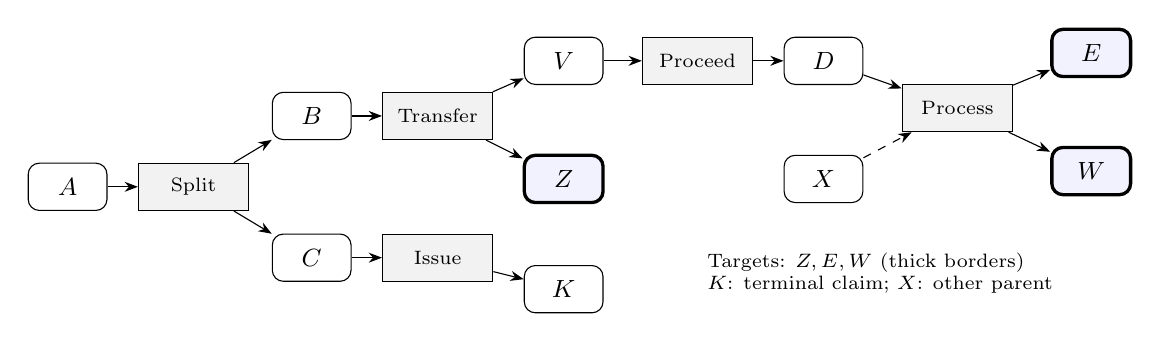
\begin{tikzpicture}[x=1cm,y=1cm,>=Stealth,
 obj/.style={draw,rounded corners,minimum width=10mm,minimum height=6mm,font=\small},
 ev/.style={draw,fill=gray!10,minimum width=14mm,minimum height=6mm,font=\scriptsize},
 target/.style={obj,very thick,fill=blue!5}]
 \node[obj] (a) at (0,0) {$A$};
 \node[ev] (s) at (1.6,0) {Split};
 \node[obj] (b) at (3.1,.9) {$B$};
 \node[obj] (c) at (3.1,-.9) {$C$};
 \node[ev] (t) at (4.7,.9) {Transfer};
 \node[obj] (v) at (6.3,1.6) {$V$};
 \node[target] (z) at (6.3,.1) {$Z$};
 \node[ev] (p) at (8,1.6) {Proceed};
 \node[obj] (d) at (9.6,1.6) {$D$};
 \node[obj] (x) at (9.6,.1) {$X$};
 \node[ev] (pr) at (11.3,1) {Process};
 \node[target] (e) at (13,1.7) {$E$};
 \node[target] (w) at (13,.2) {$W$};
 \node[ev] (is) at (4.7,-.9) {Issue};
 \node[obj] (k) at (6.3,-1.3) {$K$};
 \foreach \from/\to in {a/s,s/b,s/c,b/t,t/v,t/z,v/p,p/d,d/pr,pr/e,pr/w,c/is,is/k}
   \draw[->] (\from)--(\to);
 \draw[->,dashed] (x)--(pr);
 \node[font=\scriptsize,anchor=west,align=left] at (8,-1.1)
 {Targets: $Z,E,W$ (thick borders)\\$K$: terminal claim; $X$: other parent};
\end{tikzpicture}
\caption{Worked accounting flow after accepted production and transfer. The dashed edge is an actual input edge outside the forward traversal from $A$; the figure shows it only to explain the process accounting.}
\label{fig:worked-flow}
\end{figure*}

\subsection{선행·후속 추적}

추적은 확정된 하나의 원장 시점을 기준으로 한다.
원장 시작부터 그 시점까지의 기록 구간을 $H_t$라 쓰며,
확정 블록 해시 또는 그에 대응하는 수락 순서로 특정한다.
모든 조회는 같은 원장·시점에서 수행하고, 복호화에는 외부 승인 후
복원한 유효 감사키를 사용한다. 감사 기록의 전체 값 목록을 복호화한 뒤
거래 형식에 따라 부모 참조와 미래 식별자로 나눈다.
필요한 자료를 확인하지 못하면 추적을 실패로 처리하며,
이를 빈 경로나 미소비 상태로 간주하지 않는다.

\emph{선행 추적}(\Alg{TraceBackward})은 사용된 원료를 거슬러 올라가는 절차다.
객체의 생성 기록을 읽고, 그 기록에 암호화된 실제 부모 목록을 연다.
각 부모의 생성 기록으로 이동하는 일을 초기 등록까지 반복한다.
어떤 출력의 생성 기록을 읽었다고 해서 그 기록의 다른 출력까지
선행 경로에 포함하지는 않는다.

\emph{후속 추적}(\Alg{TraceForward})은 그 근거를 어디에 썼는지 따라가는 절차다.
객체의 생성 기록에서 미래 소비 식별자를 열고 소비 기록을 조회한다.
0이면 아직 쓰이지 않은 객체이므로 미소비 집합에 넣는다.
소비 이벤트가 있으면 타입·입력·생성 순서의 일치를 확인한다.
그 기록의 복호화된 부모 목록에도 현재 객체가 있는지 검사하고,
그 이벤트의 모든 출력으로 이어간다.
Claim과 출력 없는 종료는 종단으로 기록한다.

후속 추적은 분할·병합·가공에서 도달한 모든 출력을 포함한다.
폐기물이나 질량 0 출력도 뺄 수 없다.
다만 합류한 거래의 다른 입력을 거슬러 올라가지는 않는다.
그림의 $X$가 그 예다. 객체에서 시작하면 그 객체 하나,
기록에서 시작하면 그 기록의 전체 출력을 출발점으로 삼는다.
기록 시작의 선행·후속 그래프와 재방문 처리의 정확한 규칙은
부록~\ref{app:trace-details}에 명시한다.

결과에는 복원한 그래프와 미소비 회계 증표 $F_N$,
미해결 이전 증표 $F_V$, 종단 Claim과 종료 기록을 구분해 남긴다.
미소비 집합에는 타입 참조와 소비 식별자를 함께 보관한다.
이미 동결·사용 금지 상태인 객체도 아직 소비되지 않았다면 포함한다.

\subsection{차단 대상과 집행}

감사·동결 절차(\Alg{AuditAndFreeze})는 신뢰된 상태 관리자가
선택한 시작점의 차단을 승인한 뒤 실행한다.

전체 차단 완료를 목표로 하는 운영에서는 회계 객체의 소비와 차단
해제를 일시 중단하고, 그 중단이 적용된 뒤 확정된 $H_t$를 선택한다고
가정한다. 감사 조회와 동결 거래는 중단 중에도 허용한다.
중단은 아래의 공통 확인 시점 $H_r$까지 유지한다.
먼저 $H_t$에서 상태를 바꾸지 않고 후속 추적을 마친다.
추적에 성공한 뒤 동결 대상을
\begin{equation}
 T=F_N\cup F_V,\qquad t=(r,\nu)
 \label{eq:targets}
\end{equation}
로 고정한다. 각 $t$는 객체 참조 $r$와 소비 식별자 $\nu$의 쌍이다.
대상은 전체 미소비 집합과 정확히 같아야 한다.
이미 차단된 객체, 폐기물, 질량 0 객체와 집행에 실패한 객체도
대상 목록에 유지한다. Claim과 종료는 종단으로 남긴다.
대상이 비면 해당 시점에 차단할 미소비 객체가 없는 것으로 보고한다.

활성 대상에는 동결 거래를 제출하고, 이미 동결 또는 사용 금지된
대상은 그 차단 상태를 확인한다.
스마트 계약은 상태 관리자 권한, 타입별 식별자의 형식,
현재 미소비 여부와 허용 상태 전이를 검사한다.
감사자는 복호화한 결과에서 실제 객체의 식별자를 선택하고
전체 미소비 집합을 대상으로 유지할 책임을 맡는다.
대상별 오류 처리와 결과 형식은 부록~\ref{app:freeze-execution}에 둔다.

\subsection{차단 완료 판정}

집행을 마치면 전체 대상이 함께 차단되어 있는지 확인한다.
이를 위해 하나의 확정 시점 $H_r$에서 모든 대상을 다시 조회한다.
$H_r$은 $H_t$ 이후 또는 같은 시점이고, 같은 원장의 사용한 관찰과
거래 처리 결과를 포함해야 한다.

대상 $t$의 타입을 $\kappa_t$, 식별자를 $\nu_t$라 하자.
차단 상태 $\B$는 아직 소비되지 않았고 동결 또는 사용 금지인 경우다.
\begin{equation}
 \begin{aligned}
 \B_{H_r}(t)\ \Longleftrightarrow\quad
 &\spend^{\kappa_t}_{H_r}[\nu_t]=0\\
 {}\land\quad
 &\stat^{\kappa_t}_{H_r}[\nu_t]\in\{\stFrozen,\stRevoked\}.
 \end{aligned}
 \label{eq:blocked}
\end{equation}
\Alg{COMPLETE\_AT\_CHECKPOINT}는 다음 세 조건이 모두 맞을 때만 반환한다.
\begin{enumerate}
\item 후속 추적이 성공했고, 비어 있지 않은 전체 $T$가 대상 목록과
대상별 결과에 정확히 유지된다.
\item 위 조건에 맞는 공통 $H_r$을 확보했고,
제출 여부·처리 결과가 불명확한 거래가 없다.
\item $H_r$에서 모든 $t\in T$가 식~\eqref{eq:blocked}를 만족한다.
\end{enumerate}
정상 추적과 비어 있지 않은 $T$를 얻었지만 이 조건을 만족하지 못하면
\Alg{INCOMPLETE}로 보고하며 전체 대상과 대상별 결과를 보존한다.

완료는 $H_r$의 차단 상태에 관한 판정이며,
후속 소비는 차단이 유지되는 동안 거부된다.
전체 절차는 외부 감사와 여러 원장 거래를 연결해 수행한다.

\section{보안 분석}
\label{sec:security}
\label{sec:analysis}

이 절은 세 질문을 다룬다. 정상 요청은 제대로 처리되는가,
틀린 거래나 결과를 성공으로 받아들일 수 있는가,
공개 원장을 보는 외부인이 숨긴 자료를 구별할 수 있는가이다.
이를 각각 정확성·건전성·프라이버시로 분석한다.

건전성에서는 참여자들이 공모해 잘못된 거래·증명·문서를 제출할 수
있다고 본다. 프라이버시에서는 정직하게 생성된 공개 이력을 읽는
외부 관찰자를 다룬다. 두 성질의 공격자 범위가 서로 다르다.
감사자는 신뢰된 주체로 두며, 프라이버시 보장은 비밀을 아는
거래 당사자나 승인된 감사자에게 적용하지 않는다.

결과는 다음 신뢰 가정 아래 성립한다. 원장의 권한 판정·현재 상태 검사·
원자적 갱신과 확정 이력의 인증 조회는 정확하고,
감사자와 상태 관리자는 신뢰된다고 둔다.
외부 절차는 유효한 감사키를 제공한다.
현실 입력의 진실성이나 키 전달 서비스 자체의 보안을 증명하는 것은 아니다.

암호 방식에는 증명의 근거 입력을 분석에서 확보할 수 있는 성질,
개방값의 결합성, 등록 증명의 건전성, 해시 충돌 저항성,
소유권 비밀의 유일한 표현과 허용 난수에서의 복호화 정확성을 요구한다.
분석의 공격자는 보안 매개변수에 대한 다항 시간·질의 수로 제한한다.
각 $\epsilon$은 해당 가정의 실패 가능성에 대한 전체 실행의 상계다.
정확한 공격 규칙·가정과 상세 증명은 부록~\ref{app:security-details}에 둔다.
정리는 이 가정들을 만족하는 구성에 적용된다.
실제 암호 설정·회로와의 대응은 \ref{sec:implementation-limits}절의
구현 검증 과제로 구분한다.

\subsection{정확성}
\label{sec:correctness-proof}

정확성은 규칙을 지킨 요청이 기대한 결과를 내는 성질이다.
사용 가능한 입력으로 올바른 분할 증명을 제출하면 두 출력을 기록하고,
정상 발급 문서의 공개 검증은 통과해야 한다.
필요한 기록과 유효 키가 있고 인증 조회가 끝나면,
고정 $H_t$의 추적도 정확한 이력과 미소비 집합을 반환해야 한다.

동결의 완료에는 추가 조건이 필요하다.
비어 있지 않은 전체 대상 $T$가 $H_t$부터 공통 $H_r$까지
소비되지 않고, 이미 차단된 대상과 새 동결의 차단 상태가 유지되어야 한다.
필요한 합법적 동결·조회·거래 결과와 공통 시점 확인도 정한 유한
한도 안에 확보해야 한다. 대상이 비면 빈 대상 결과를 반환한다.
경합이나 자료 부재가 있는 실행에 성공을 약속하는 정의는 아니다.

\textbf{정리 1 (Correctness).}
이 정상 조건 아래 정직 증명을 최대 $Q$회 생성하고,
한 번의 증명 완전성 실패 확률이 $\epsilon_{\rm comp}$ 이하이면
\begin{equation}
 \Pr[\mathsf{Fail}_{\rm corr}]
 \leq Q\epsilon_{\rm comp}+\epsilon_E+\epsilon_H.
 \label{eq:correctness-bound}
\end{equation}
이다. $\mathsf{Fail}_{\rm corr}$는 정상 조건이 성립하는 요청이
기대한 결과를 내지 못한 사건이다.
$\epsilon_E,\epsilon_H$는 전체 실행의 복호화 실패와 관련 해시
충돌의 상계다. 이는 정상 조건과 실패가 함께 생기는 확률이며,
정상 조건을 만족한 실행만 골랐을 때의 실패 비율은 아니다.

\emph{증명의 요지.}
올바른 증명은 검증을 통과하고, 유효한 실행 조건은 정해진 상태
갱신을 허용한다. 감사 암호문을 정확히 열면 실제 부모와 미래
식별자를 얻으므로 연결을 따라 정확히 추적한다.
동결의 추가 조건은 전체 대상의 공통 시점 차단을 보장한다.
따라서 실패는 증명 완전성·복호화·관련 해시 가정의 실패 중
하나를 필요로 한다. 세 가능성을 합하면 위 상계를 얻는다.
부록~\ref{app:correctness-details}는 정상 조건과 사건을 구체화한다.

\subsection{건전성}
\label{sec:soundness-proof}
\label{sec:binding-argument}

건전성은 틀린 거래나 결과를 올바른 것으로 받아들이기 어려운 성질이다.
여기서는 실제 생성 값과 다른 거래, 잘못된 추적 성공,
거짓 전체 완료와 차단 유지 중의 후속 소비를 하나의 실행에서 다룬다.
자료 부족의 명시적 실패나 대상을 보존한 \Alg{INCOMPLETE}는
공격 성공이 아니다.

\textbf{정리 2 (Soundness).}
부록~\ref{app:soundness-details}의 암호 가정과 위 신뢰 모델 아래
\begin{equation}
 \Pr[\mathsf{Exp}_{\rm sound}=1]\leq
 \epsilon_B:=\epsilon_X+\epsilon_C+\epsilon_M+\epsilon_H+\epsilon_E.
 \label{eq:bad-binding-bound}
\end{equation}
이다. $\epsilon_X,\epsilon_C,\epsilon_M,\epsilon_H,\epsilon_E$는
각각 증인 추출, 개방값 결합, 포함 관계, 관련 해시 충돌,
복호화의 전체 실행 실패 상계다.
증인 추출은 증명의 근거를 분석에서 확인하는 권한이며,
일반 검증자에게 비공개 자료를 공개한다는 뜻은 아니다.

\paragraph{거래와 추적의 일치.}
\label{sec:trace-argument}

증명의 첫 단계는 등록 때의 실제 값을 기준으로 거래를 확인하는 것이다.
수락된 증명의 근거 입력을 얻었을 때, 그것이 등록 때의 값과 다르면
개방값 결합성이 깨진다. 값과 적법한 소유 비밀이 같으면 소비
식별자도 같으므로, 현재 소비·상태 검사가 바로 그 객체에 적용된다.
감사 암호문도 같은 입력·출력에서 계산되므로 실제 부모와 미래
식별자를 돌려준다. 공개 Claim 검증의 문서·정책 연결도 같은 방식으로 다룬다.

다음으로 이 연결을 한 단계씩 따라간다.
실제 생성·소비 이력으로 정의한 그래프를 기준으로 삼으며,
감사 결과 자체를 정답으로 정의하지 않는다.
미래 식별자의 소비 기록이 0이면 정확히 미소비인 객체이고,
소비 기록이 있으면 실제 소비 이벤트의 전체 출력으로 이동한다.
이 과정을 반복하면 정해진 후속 경로와 미소비 집합을 얻는다.
선행 추적은 실제 부모를 거슬러 올라간다.
자료가 없거나 일관성이 깨지면 성공한 결과를 내지 않는다.
형식적인 시작점과 간선의 정의는 부록~\ref{app:trace-details}와 같다.

\paragraph{전체 차단의 보장.}

$T$를 $H_t$에서 찾은 전체 미소비 회계 증표·미해결 이전 증표로 두자.
공통 $H_r\geq H_t$에서 다음 조건이 성립한다고 하자.
\begin{equation}
 T\ne\varnothing,\qquad
 \forall t\in T:\ \B_{H_r}(t).
 \label{eq:frontier-cut}
\end{equation}
이는 대상이 비어 있지 않고 모두 미소비·차단 상태라는 뜻이다.
후속 사용을 계속하려면 남은 기록 중 적어도 하나를 먼저 써야 한다.
$H_t$ 이후 최초의 그런 사용이 있었다면 $T$의 객체 하나가 소비됐어야
하므로, $H_r$에서 모두 미소비라는 조건과 모순된다.
$H_r$ 이후에도 $T$의 차단이 유지되면 모든 소비 경로의 현재 상태
검사가 그 첫 사용을 거부한다. 다른 정상 입력과 합치는 거래도
차단된 입력의 검사를 피할 수 없다.

이 논증에 V절의 전체 대상·공통 시점·거래 결과 확인을 적용하면
거짓 전체 완료도 배제된다. 전이·추적·완료의 실패는 같은 암호
가정의 실패 집합에 포함되므로 상계를 세 번 더하지 않는다.
완료 보고와 오류가 함께 발생하는 확률의 상계이며,
완료를 보고한 실행만 고른 조건부 오류율은 아니다.

V절의 동결·해제 사례는 공통 시점 없이 완료를 보고하면 안 되는 이유다.
동결 전에 소비된 대상을 목록에서 빼는 것도 남은 파생 기록을 놓치게 한다.
반대로 \Alg{INCOMPLETE}라고 해서 현재 쓸 수 있는 후속 객체가
반드시 있다는 뜻은 아니다. 대상이 종료로 소진됐거나 다른 실행이
파생 객체를 이미 막았을 수도 있다.
이 결과는 본 절차의 충분조건이며 모든 차단 방식의 필요조건은 아니다.

\subsection{프라이버시}
\label{sec:privacy-proof}

프라이버시는 숨긴 수치나 입력 연결은 다르지만,
공개하기로 한 정보는 같은 두 이력을 외부인이 구별하기 어려운 성질이다.
예를 들어 거래 종류와 공개 제품 주장이 같은 두 유효한 이력에서,
실제로 쓴 원료 기록의 연결이나 비공개 수치가 다를 수 있다.
다른 공개 조건도 같다면 외부인이 어느 이력인지 알아내기 어려워야 한다.
거래 종류·정책·입출력 형상·호출자·시간·기한·공개 Claim과
공개 색인의 동일성 같은 정보는 보호 대상에서 제외한다.
정확한 공개 범위는 부록~\ref{app:privacy-details}에 명시한다.

대상은 독립적인 정직 난수로 생성된 이력을 읽는 수동 외부 관찰자다.
설정 전에 고정한 $K-1$개 이하 위원회 조각은 볼 수 있지만,
참여자 비밀·개방값, $SK_B$, 보호 관계의 감사·상태 공개는 받지 않는다.
능동 거래 제출·복호화 질의도 제외한다.
따라서 승인된 감사자나 비밀을 아는 거래 당사자까지 보호하는 주장은 아니다.

분석에서는 용도가 다른 해시를 독립된 이상적 무작위 함수로 다루는
무작위 오라클 모형을 사용한다.
두 키 암호화의 기밀성과 여러 증명을 함께 보아도 성립하는 영지식
성질도 가정한다.

\textbf{정리 3 (Privacy).}
부록~\ref{app:privacy-details}의 게임과 충분조건 아래
\begin{equation}
 \mathsf{Adv}_{\rm hist}\leq
 2(\epsilon_Z+\epsilon_A+\epsilon_D+\epsilon_{\rm RO}).
 \label{eq:privacy-bound}
\end{equation}
이다. $\epsilon_Z$는 전체 증명의 영지식 구별 이득,
$\epsilon_A,\epsilon_D$는 임계 키 보호와 데이터 암호화의 구별 이득이다.
$\epsilon_{\rm RO}$는 숨은 입력 추측·관련 충돌의 상계다.
각 이득은 두 실험을 구분할 수 있는 정도를 나타낸다.

\emph{증명의 요지.}
공개 증명을 비공개 입력 없이 만들 수 있는 분석용 자료로 바꾸고,
키 보호·감사 암호문의 내용을 대체한 뒤,
숨은 기록과 식별자를 독립된 무작위 값으로 바꾼다.
각 변화를 구별할 수 있으면 해당 가정도 깨뜨릴 수 있다.
마지막에 남는 분포는 공개 정보에만 의존하므로 두 이력은 구별하기 어렵다.
독립 키, 비밀·난수의 범위, 공개 자료의 재현과 각 변경 순서에 필요한
조건은 부록에서 확인한다.

\section{검증 및 실험 평가}
\label{sec:evaluation}

이 절은 프로토콜 구성과 조건부 분석을 보완하여 두 가지를 확인한다.
첫째, 기록을 따라가고 남은 대상을 차단하는 동작이 맞는가.
둘째, 거래와 감사에 얼마나 많은 계산·원장 작업·시간이 필요한가.
먼저 측정 방법을 설명하고, 동작과 비용의 결과를 제시한 뒤
기존 연구와 비교할 수 있는 범위를 정리한다.

\subsection{실험 환경 및 방법}

Table~\ref{tab:evidence-scope}는 보안 분석과 평가 근거의 역할을
구분한다. 기호 모델은 정해진 사례의 논리 동작을, 시제품 실행은
대표 경로의 연결을, 성능 자료는 선택한 조건의 비용을 보여 준다.
이들은 동일한 판본을 사용한 하나의 통합 검증 결과가 아니다.

\begin{table}[ht]
\centering\small
\caption{Scope of the analysis and evaluation evidence}
\label{tab:evidence-scope}
\begin{tabularx}{\columnwidth}{@{}>{\raggedright\arraybackslash}p{.19\columnwidth}Y@{}}
\toprule
Evidence & Supported result and boundary \\ \midrule
Proofs & Conditional correctness, soundness, and passive privacy; no concrete conformance result. \\
Symbolic model & Selected accounting, tracing, and completion cases; no cryptographic execution or full specification validation. \\
Prototype & Selected paths at \texttt{8560fd3}; test verifier and single audit-key version. \\
Costs & Measured workload costs; independent-run variability and some version/configuration mappings remain unresolved. \\
\bottomrule
\end{tabularx}
\end{table}

성능 측정 환경은 Table~\ref{tab:eval-env}와 같다.
회로는 PLONK-KZG와 BLS12-381을 사용하고, 감사 암호화에는
Jubjub와 Poseidon2를 사용한다. 원장 실행 환경은 로컬 Anvil이다.
기호 검사, 고정된 시제품 판본의 실행 기록과 성능 측정 자료는
평가 아티팩트에 정리되어 있다~\cite{zkdpp-evaluation-artifact-2026}.

\begin{table}[ht]
\centering\small
\caption{Performance measurement environment}
\label{tab:eval-env}
\begin{tabularx}{\columnwidth}{@{}lY@{}}
\toprule
Item & Configuration \\ \midrule
Host & MacBook Pro (MacBookPro18,1) \\
OS & macOS 26.3 (25D125) \\
CPU & Apple M1 Pro, 10 cores (8 performance + 2 efficiency) \\
Memory & 32 GB \\
Circuit libraries & gnark 0.15.0; gnark-crypto 0.20.1 \\
Proof / curve & PLONK-KZG / BLS12-381 \\
Audit curve / hash & Jubjub / Poseidon2 \\
Ledger node & Anvil 1.7.1 \\
Compiler / EVM & Solidity 0.8.30 / Prague \\
\bottomrule
\end{tabularx}

\end{table}


비용은 세 지표로 본다. \emph{제약 수}는 증명 회로에 표현한
계산 조건의 수다. \emph{gas}는 원장이 거래를 처리할 때 수행한
작업량을 나타내는 단위로, 지불 금액 자체는 아니다.
성공한 거래 영수증의 \texttt{gasUsed} 값을 사용한다.
\emph{전체 실행 시간}(E2E)은 비공개 입력을 준비하기 시작한 때부터
거래가 성공했다는 영수증을 확인할 때까지의 시간이다.
세 지표가 측정하는 작업은 서로 다르다.
감사 유무 비교에서는 같은 종류의 거래에 대해 입력·상태·권한·트리
조건을 맞추고, Process 실험에서는 상태 합을 고정한 채 입출력
개수를 바꾼다. 추적의 작업량은 중복을 제외한 방문 감사 기록 수,
동결의 작업량은 대상 수이다. 두 작업은 별도로 측정하므로
그 시간을 합산한 전체 감사 지연은 제시하지 않는다.

기호 모델은 암호 계산을 직접 실행하는 대신, 기록과 연결에
이름을 붙여 규칙을 검사하는 작은 프로그램이다.
선택한 유한 사례에서 회계·추적·완료 조건이 맞는지 확인한다.
시제품의 대표 기능 검증은 커밋 \texttt{8560fd3}의 실행 기록과
제한 테스트를 사용한다. 이 판본의 원장 시나리오는 실제 증명의
유효성을 검사하지 않는 시험용 검증기로 거래를 생성한다.
감사키도 단일 키 판본이므로 현행 두 키 구성의 검증과 구분한다.
회로 제약 검사는 별도로 제시한다.

시간 지표는 관측된 실행값으로 제시한다. 키 복구는 준비 실행 후
공식 측정 한 번에 포함된 1,000회 내부 복구의 평균이며,
그 밖의 시간에는 별도 실행을 몇 번 반복했고 결과가 얼마나
달랐는지에 관한 자료가 없다. 따라서 시간 값은 관측한 실행의
비용이며, 반복 실행의 안정성을 나타내는 통계는 아니다.
추가 확인이 필요한 근거는 \ref{sec:implementation-limits}절에 모았다.

\subsection{시스템 동작 및 성능 평가}

동작 검사는 문제 원료의 근거가 여러 갈래로 나뉜 사례에서 시작한다.
어떤 기록을 찾아야 하고 무엇을 막아야 하는지 먼저 확인한다.
그 뒤 거래 종류별 비용, 감사 기능의 추가 비용과
작업 규모·전달 방식·공정 입출력 수에 따른 변화를 살펴본다.

% Symbolic validation component of Evaluation.
\label{sec:model-validation}

이 검사 프로그램은 거래에 들어온 기록과 새로 나온 기록의
관계, 기록의 소비 여부와 동결 상태만 Python 3의 자료구조로
표현한다. 암호문과 소비 식별자는 실제 암호 연산 대신
서로 구별되는 이름표로 나타낸다. 영지식증명·암호화·인증이나
원장 거래는 실행하지 않는다.

추적 결과를 확인하기 위해 같은 이력을 두 방식으로 계산했다.
첫째는 제안한 감사 절차처럼 감사 자료와 소비 여부를 조회해
연결된 기록을 찾는다. 둘째는 거래마다 적어 둔 입력·출력
목록만으로 연결 관계를 새로 만든 뒤, 도달할 수 있는 기록을
모두 찾는다. 둘째 계산은 첫째 계산의 결과를 사용하지 않는다.
분기·합류·발급·종료, 이전 회수, 질량 0 출력 등을 포함한
네 개의 정해진 거래 이력을 사용했다. 각 이력에서 거래가
하나씩 추가되는 모든 시점마다, 그때 존재하는 기록과 거래를
각각 출발점으로 삼아 앞뒤 추적 결과를 비교했다.
기록·연결·아직 소비되지 않은 대상에 대한 비교 334건에서
두 방식의 결과가 일치했다~\cite{zkdpp-symbolic-model-2026}.
하지만 두 방식이 같이 틀리면 이 비교로 발견할 수 없다.
실제로 Entry 거래 자체에서 후속 추적을 시작하면 둘 다
Entry를 결과에 넣는다. 명세에서는 Entry의 출력부터
포함해야 한다. 따라서 334건의 일치가 명세 전체와의
일치를 뜻하지는 않는다.

그림~\ref{fig:worked-flow}의 원료 $A$에서 추적을 시작하면
아직 소비되지 않아 동결해야 할 대상은 $Z,E,W$다.
합류 거래에 함께 들어온 다른 원료 $X$의 과거로는
거슬러 올라가지 않는다. 이미 발급된 $K$도 더 소비할
수 없으므로 동결 대상이 아니다. 반면 $Z$는 질량이 0이고
$W$는 폐기물이지만 둘 다 아직 소비할 수 있어 포함된다.
$V$가 인수되기 전 시점에서는 대상이 $C,V,Z$다.
감사를 시작한 뒤 $V$가 먼저 인수되더라도, 처음 정한
대상 목록에서 $V$를 빼지 않는다. 동결을 마치지 못한 것으로
보고한다.

전체 검사 408건에는 앞의 추적 비교 334건과
동결 상태·오류 처리·회계 규칙 검사가 포함된다.
정해진 사례에서 동결되거나 사용 금지된 기록을 거래 입력으로
쓰면 거부했고, 이전 증표의 인수와 회수 중 먼저 수락된
한쪽만 그 증표를 소비할 수 있었다. 감사 자료가 빠지거나
형식이 틀리면 추적이 실패했다. 동결 대상이 빠졌거나
일부만 동결된 경우, 제출 결과가 불분명하거나 동결 전에
대상이 소비된 경우에는 완료를 보고하지 않았다.
각 대상의 동결 영수증이 따로 존재해도 모든 대상이
\emph{같은 시점에} 차단된 적이 없으면 완료로 보지 않았다.
질량 0 가공 출력에 탄소 잔여를 주려는 이전 사례는 거부하고,
잔여가 양의 질량 출력에 배분되는지 확인했다. 서로 다른 소유
비밀이 같은 소유자를 나타내는 사례는 식별자 가정의 한계를
보여 주었다.

이 검사는 정해진 몇 가지 사례에서 규칙의 동작을 살펴본
것이다. 실제 암호·원장 구현이 명세를 따른다는 증거도,
모든 가능한 거래 이력에서 올바르게 작동한다는 증거도 아니다.


\paragraph{시제품의 추적·차단 실행.}
시제품의 대표 시나리오는 $A\rightarrow(B,C)$,
$B\rightarrow(D,E)$로 분기된 이력이다.
감사자는 $A$에서 미소비 대상 $C,D,E$를 찾고 각 대상의 동결을
요청한 뒤 최종 상태를 확인한다. 저장된 Anvil RPC 결과에는
기준 블록 7, 대상 3개, 동결 거래 3건과 확인 블록 10이 기록되어
있으며, 결과는 \Alg{COMPLETE\_AT\_CHECKPOINT}이다.
이는 해당 분기 그래프에서 조회·복호화·추적·동결·결과 확인이
연결된 실행 근거이다.

Table~\ref{tab:eval-functional}은 이 실행과 제한 테스트의 결과를
대표 경로·시험 조건별로 정리한다.

\begin{table*}[t]
\centering\small
\caption{Prototype functional checks and their evidence scope}
\label{tab:eval-functional}
\begin{tabularx}{\textwidth}{@{}>{\raggedright\arraybackslash}p{35mm}YY@{}}
\toprule
Check & Observed result & Evidence scope \\ \midrule
Branch tracing and freezing & $C,D,E$ recovered; 3 freeze transactions; checkpoint completion & Archived Anvil RPC run; test verifier \\
Entire target set & 3 targets and 3 freeze calls; complete & Memory-backed test \\
Trace failure & No freeze calls; trace failure & Failure-path test \\
Consumption before freeze & Consumed target retained; incomplete & Failure-path test \\
Valid circuit inputs & 10 representative relations satisfy constraints & Compilation, public-input and IsSolved tests \\
\bottomrule
\end{tabularx}
\par\smallskip\begin{minipage}{\textwidth}\footnotesize Prototype commit 8560fd3; archived tests from 9 September 2026. A test verifier does not validate real proofs.\end{minipage}
\end{table*}


\paragraph{기본 거래와 감사 추가 비용.}
Table~\ref{tab:eval-events}는 감사 기능을 포함한 아홉 거래의
비용이다. 제약 수는 18,115--55,402개, gas는
534,277--3,577,414, E2E는 674.484--1,497.729\,ms로 나타났다.
Process의 제약 수, Transfer의 gas, Split의 E2E가 각각 가장
컸다. 한 지표가 가장 크다고 다른 지표도 가장 큰 것은 아니다.
증명에서 검사할 계산, 원장에 기록할 작업과 전체 처리 시간이
서로 다르기 때문이다.

\begin{center}
\begin{minipage}{\columnwidth}
\centering\small\captionsetup{hypcap=false}
\captionof{table}{감사 자료를 포함한 거래별 비용}
\label{tab:eval-events}
\begin{tabular*}{\columnwidth}{@{\extracolsep{\fill}}lrrr@{}}
\toprule
거래 & 제약 수 & gas & E2E (ms) \\ \midrule
Entry & 18,115 & 2,258,715 & \shortstack[r]{770.834\\\scriptsize[750.529, 881.576]} \\
Transfer & 49,883 & 3,577,414 & \shortstack[r]{1,464.369\\\scriptsize[1,349.669, 1,541.041]} \\
Proceed & 35,858 & 1,784,082 & \shortstack[r]{1,278.965\\\scriptsize[1,213.766, 1,330.913]} \\
Recall & 35,987 & 1,785,084 & \shortstack[r]{1,250.315\\\scriptsize[1,193.623, 1,527.191]} \\
Merge & 51,543 & 1,888,301 & \shortstack[r]{1,361.248\\\scriptsize[1,243.049, 1,687.575]} \\
Split & 48,608 & 2,730,046 & \shortstack[r]{1,497.729\\\scriptsize[1,333.420, 1,564.472]} \\
Process & 55,402 & 1,866,617 & \shortstack[r]{1,335.974\\\scriptsize[1,308.756, 1,417.352]} \\
Exit & 27,940 & 534,277 & \shortstack[r]{674.484\\\scriptsize[649.884, 705.232]} \\
Issue & 35,957 & 678,565 & \shortstack[r]{1,225.264\\\scriptsize[1,084.983, 1,259.957]} \\
\bottomrule
\end{tabular*}
\par\smallskip\begin{minipage}{\columnwidth}\footnotesize Process는 입력 2개·출력 1개다. 준비 1회 뒤 공식 5회의 gas·E2E 중앙값이다. E2E의 대괄호는 5회 중 최소·최대이며, 각 거래의 gas 최소·최대 차이는 24--84다. 반복별 원시 기록과 집계 코드는 공개 저장소에 제공한다~\cite{zkdpp-evaluation-data-2026}.\end{minipage}
\end{minipage}
\end{center}


Transfer의 비용을 나누어 보면 어떤 작업이 큰 몫을
차지하는지 알 수 있다. Transfer는 회계 증표 하나를 소비하고
이전 증표와 잔여 회계 증표를 생성한다. 이 거래의 제약 수는 머클 경로 검증 9,825개,
감사 암호문 검증 14,238개, 상태 범위·배분 검증 17,994개,
커미트먼트·소비 식별자·소유자 주소 계산 7,826개로,
합계 49,883개이다. 원장에서는 머클 트리 해시 계산
1,422,404 gas와 조회·저장 1,276,500 gas의 합이
2,698,904 gas로 전체의 75.44\%를 차지하였다.

감사 기능 때문에 추가되는 비용은 같은 조건에서 감사 자료를
포함한 경우(on)와 제외한 경우(off)를 빼서 구한다.
제약 수 $C$와 gas $G$에 대해
$\Delta C=C_{\rm on}-C_{\rm off}$,
$\Delta G=G_{\rm on}-G_{\rm off}$로 계산한다.
Fig.~\ref{fig:eval-audit}와 Table~\ref{tab:eval-audit}에서
추가 제약 수는 11,533--14,238개, 추가 gas는
130,705--356,287이다. off를 분모로 한 상대 증가율은
각각 31.70--202.93\%와 9.69--54.67\%이다.
Entry는 추가 제약 수가 12,135개이지만 off 값이 5,980개로
작아 상대 증가율이 202.93\%로 나타났다.

\begin{figure*}[t]
\centering
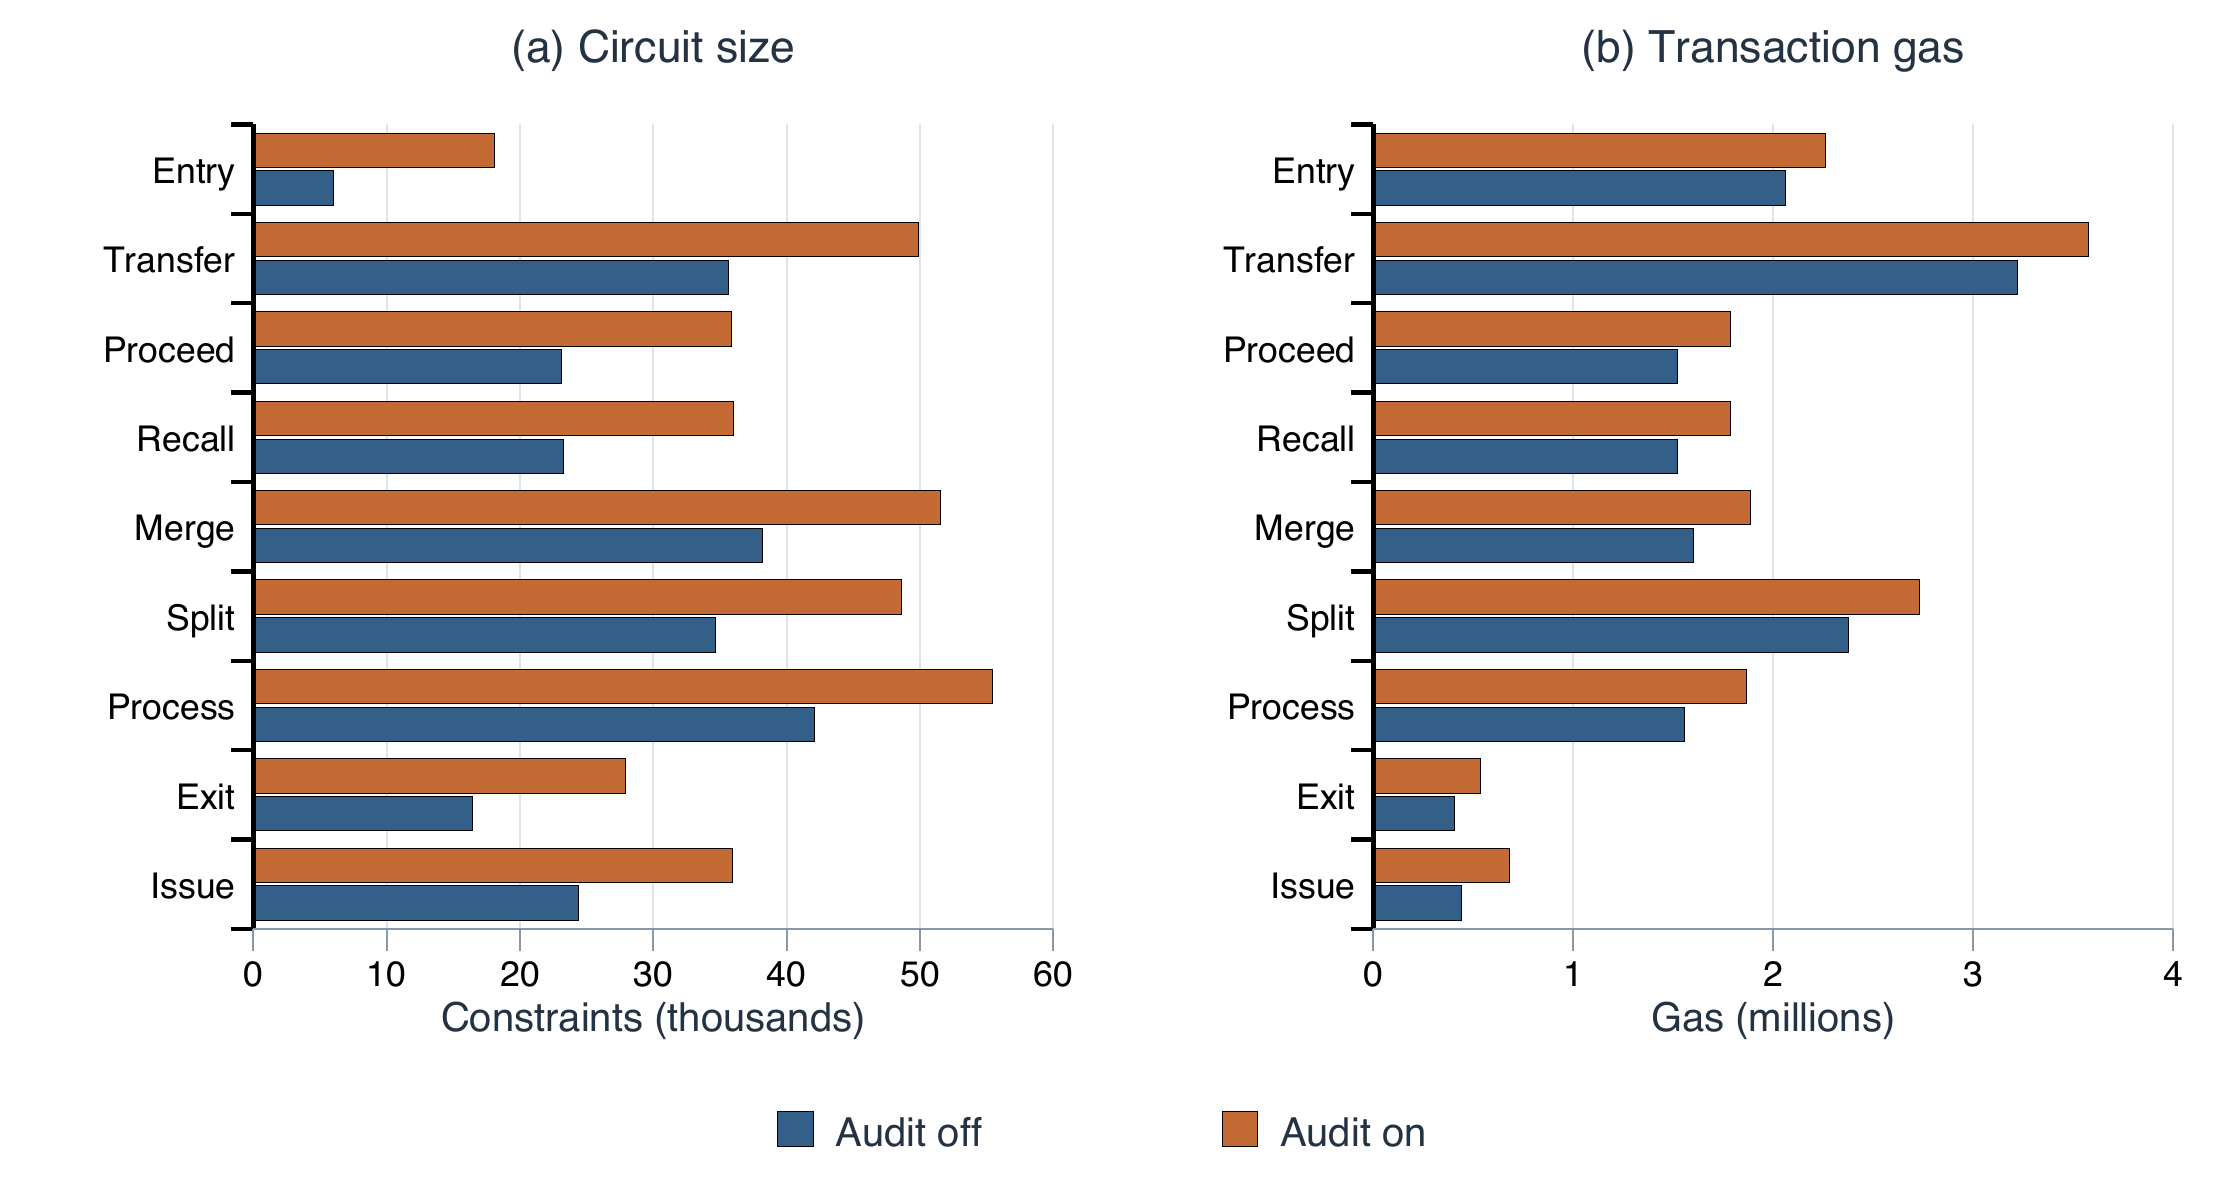
\includegraphics[width=.94\textwidth]{figures/evaluation/audit.png}
\caption{Circuit constraints and transaction gas with and without audit data. The panels use different units.}
\label{fig:eval-audit}
\end{figure*}
\begin{table*}[t]
\centering\small
\caption{Matched audit-off and audit-on costs}
\label{tab:eval-audit}
\begin{tabular*}{\textwidth}{@{\extracolsep{\fill}}lrrrrrr@{}}
\toprule
Event & $C_{\rm off}$ & $C_{\rm on}$ & $\Delta C$ & $G_{\rm off}$ & $G_{\rm on}$ & $\Delta G$ \\ \midrule
Entry & 5,980 & 18,115 & 12,135 & 2,059,123 & 2,258,715 & 199,592 \\
Transfer & 35,645 & 49,883 & 14,238 & 3,221,268 & 3,577,414 & 356,146 \\
Proceed & 23,123 & 35,858 & 12,735 & 1,519,228 & 1,784,082 & 264,854 \\
Recall & 23,252 & 35,987 & 12,735 & 1,520,722 & 1,785,084 & 264,362 \\
Merge & 38,208 & 51,543 & 13,335 & 1,599,289 & 1,888,301 & 289,012 \\
Split & 34,671 & 48,608 & 13,937 & 2,373,759 & 2,730,046 & 356,287 \\
Process & 42,067 & 55,402 & 13,335 & 1,557,348 & 1,866,617 & 309,269 \\
Exit & 16,407 & 27,940 & 11,533 & 403,572 & 534,277 & 130,705 \\
Issue & 24,424 & 35,957 & 11,533 & 438,706 & 678,565 & 239,859 \\
\bottomrule
\end{tabular*}
\par\smallskip\begin{minipage}{\textwidth}\footnotesize $C$: constraints; $G$: gas. Inputs, state, permissions and tree conditions are matched. Differences are on minus off.\end{minipage}
\end{table*}


감사 암호화를 계산할 때에는 타원곡선의 점에 정수를 곱하는
스칼라 곱셈이 사용된다. Transfer의 감사 추가 제약 14,238개 중
이 연산 두 번은
8,611개로 60.48\%를 차지하였다. 나머지는 키·마스크 계산
2,399개, 난수·암호문 검증 1,723개와 출력 소비 식별자 계산
1,505개이다. 감사 추가 gas 356,146 중 감사 기록 저장의
저장 연산 SSTORE는 324,100 gas로 91.00\%이며, 증명 검증 호출 증가분은
4,585 gas, 기타 조회·calldata 증가분은 27,461 gas이다.
따라서 이 거래에서는 두 스칼라 곱셈과 감사 자료 저장이 각각
추가 회로 비용과 추가 원장 비용의 주요 부분을 차지한다.
이 비율은 Transfer의 감사 추가 비용에 대한 분해이다.

\paragraph{추적·동결 규모와 로컬 키 복구.}
추적 규모 $V$는 고유 방문 감사 기록 수, 동결 규모 $F$는 대상
수이다. 같은 Split 시나리오에서 각 작업을 10, 100, 1,000개
규모로 측정하였다. 추적에는 기록 조회·복호화·탐색을, 동결에는
제출 전 상태 검사·대상별 거래 실행·최종 상태 확인을 포함한다.
동결 구현은 대상 하나마다 거래 하나를 제출한다.

\begin{figure*}[t]
\centering
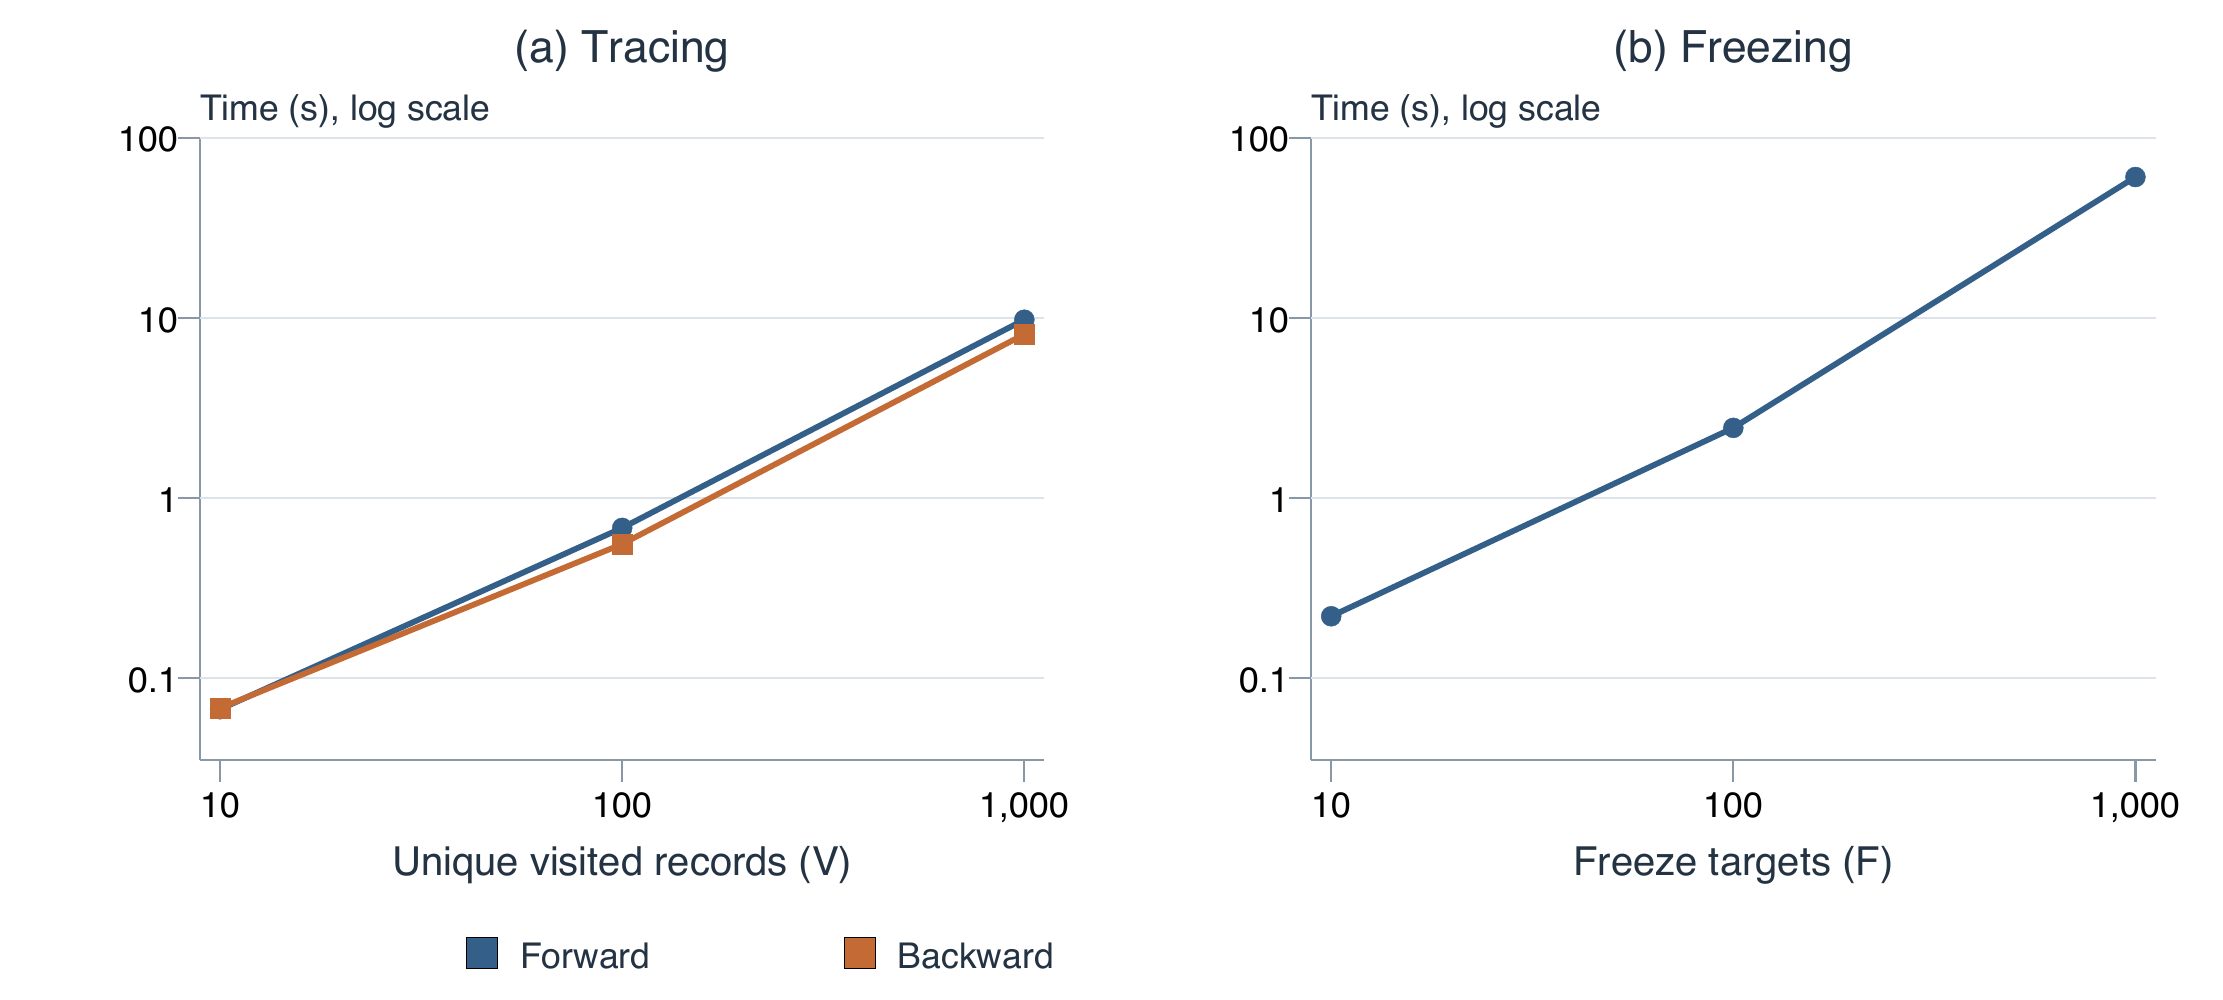
\includegraphics[width=.94\textwidth]{figures/evaluation/tracing-freeze.png}
\caption{Tracing and freezing time. Both panels use logarithmic time axes; $V$ counts visited records and $F$ counts freeze targets. Lines connect measured points.}
\label{fig:eval-trace}
\end{figure*}
\begin{table}[t]
\centering\small
\caption{Time by visited records or freeze targets}
\label{tab:eval-trace}
\begin{tabular*}{\columnwidth}{@{\extracolsep{\fill}}rrrr@{}}
\toprule
$V$ or $F$ & Forward (s) & Backward (s) & Freeze (s) \\ \midrule
10 & 0.067 & 0.068 & 0.220 \\
100 & 0.681 & 0.554 & 2.448 \\
1,000 & 9.760 & 8.102 & 60.540 \\
\bottomrule
\end{tabular*}
\par\smallskip\begin{minipage}{\columnwidth}\footnotesize $V$: unique visited audit records; $F$: freeze targets. The two tasks are measured separately on the Split scenario.\end{minipage}
\end{table}


Table~\ref{tab:eval-trace}에서 기록 1,000개의 선행 추적은
8.102초, 후속 추적은 9.760초이며, 대상 1,000개의 동결은
60.540초이다. 규모가 100에서 1,000으로 증가할 때 시간은
각각 약 14.62배, 14.33배와 24.73배가 되었다.
이 구간에서 동결의 시간 증가가 더 크게 나타났으며,
다만 세 크기만 측정했으므로 더 큰 모든 작업량에서도
어떤 비율로 시간이 늘어날지 일반화할 수는 없다.
활성 회계 증표 하나를 동결 상태로 바꾸는 거래의 gas는
49,434이다. 이는 해당 타입과 상태 전이에 대한 단일 거래의
값으로, 이전 증표나 배치 동결의 비용과 구분한다.
수행 시간 측정과 \ref{sec:audit}절의 전체 완료 조건 검증도
서로 다른 평가 대상이다.

로컬 키 복구는 위원회 공개키와 위원별 공개 조각을 사전에
검증한 뒤, 선택한 $k$개 조각을 검증하고, 조각을 수학적으로 합치는
라그랑주 보간으로 비밀값을 복구한 뒤,
그 결과가 공개키와 맞는지 확인하는 시간을 측정하였다.
전체 위원 수 $n=10$에서 $k$를 2, 3, 5, 7, 10으로 바꾸었다.
공개 자료의 사전 검증, 키 생성·분산 키 생성(DKG), 통신과 승인
대기는 측정 구간에서 제외하였다.

\begin{figure}[t]
\centering
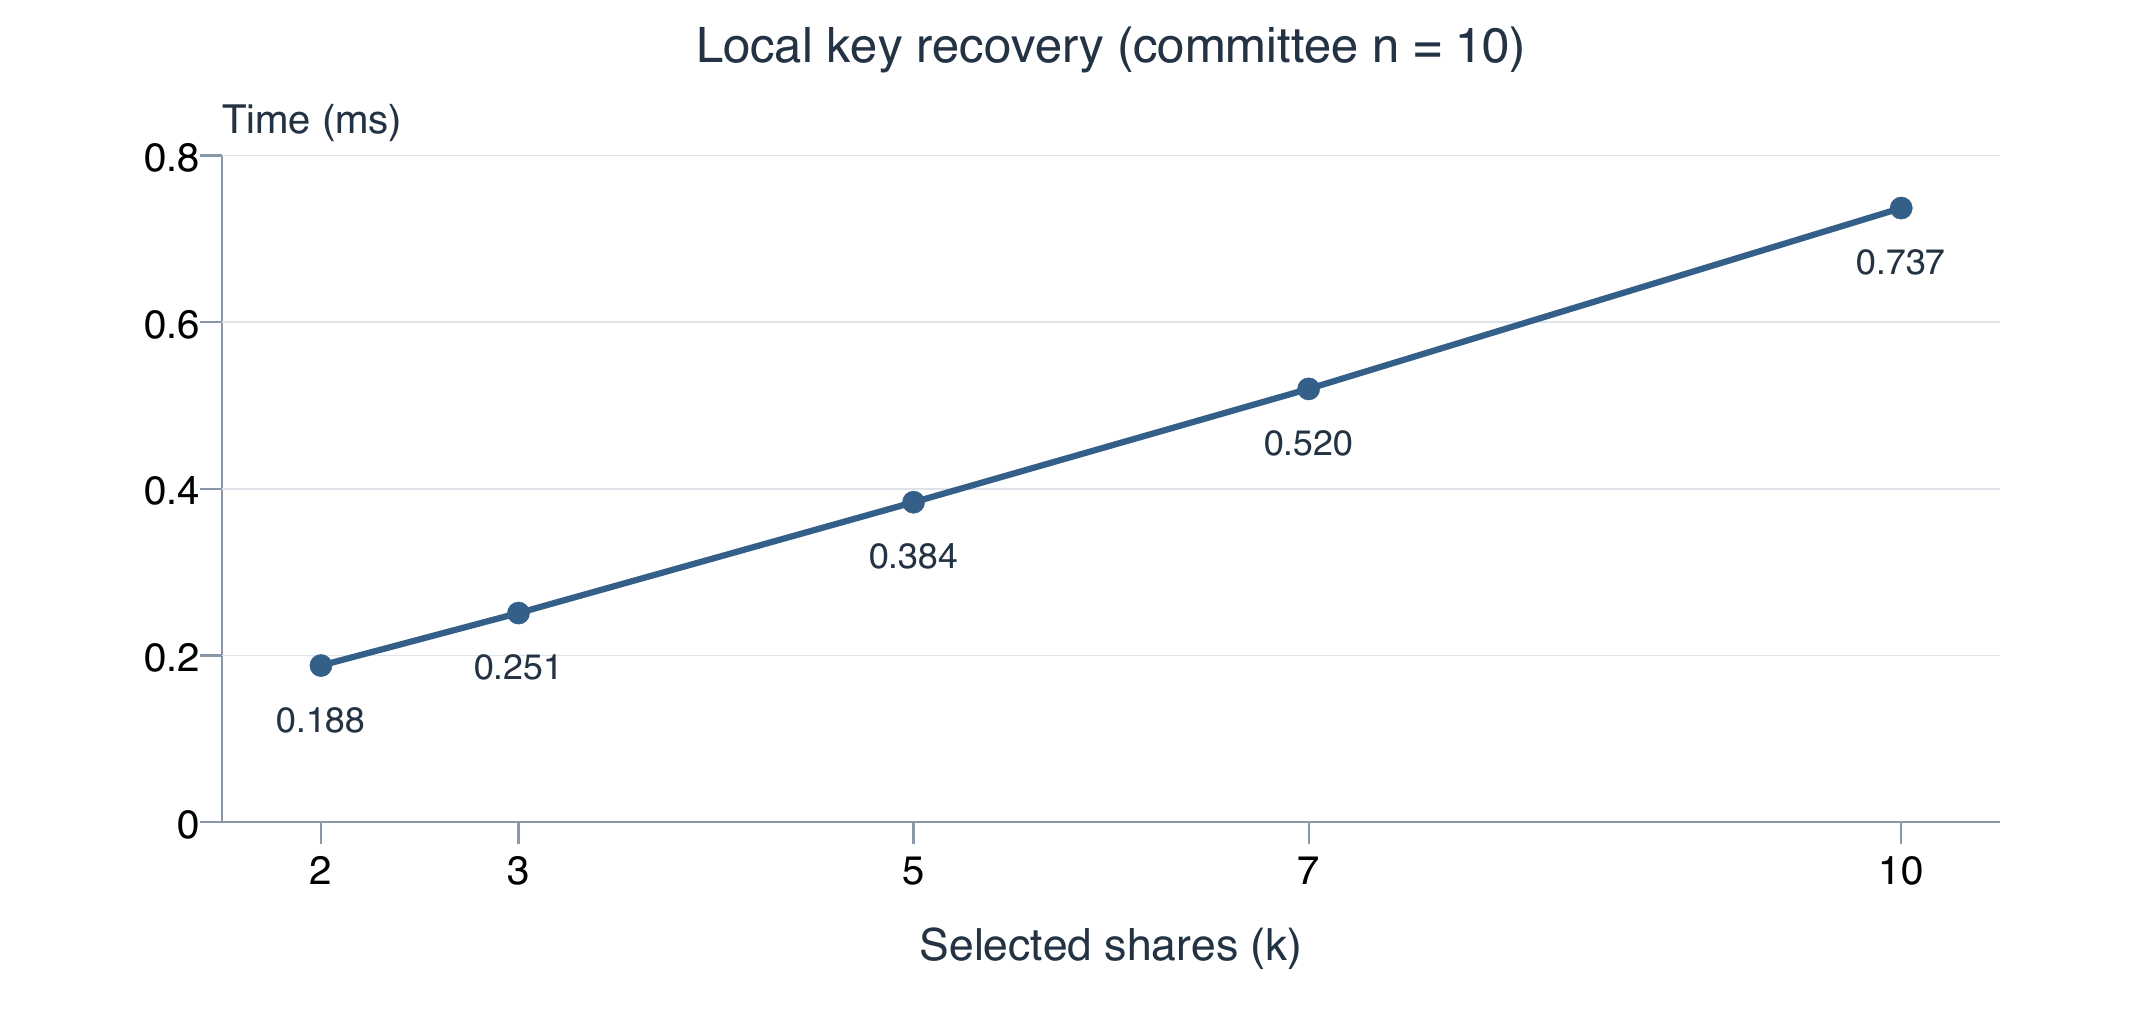
\includegraphics[width=\columnwidth]{figures/evaluation/key.png}
\caption{Local key recovery for $n=10$. Each point is the mean of 1,000 internal recoveries in one timed run after warm-up.}
\label{fig:eval-key}
\end{figure}
\begin{center}
\begin{minipage}{\columnwidth}
\centering\small\captionsetup{hypcap=false}
\captionof{table}{공개 자료 확인 후 감사 비밀키 복원 시간}
\label{tab:eval-key}
\begin{tabular*}{\columnwidth}{@{\extracolsep{\fill}}rrr@{}}
\toprule
전체 위원 수 & 사용 조각 수 & 평균 (ms) \\ \midrule
10 & 2 & 0.188 \\
10 & 3 & 0.251 \\
10 & 5 & 0.384 \\
10 & 7 & 0.520 \\
10 & 10 & 0.737 \\
\bottomrule
\end{tabular*}
\par\smallskip\begin{minipage}{\columnwidth}\footnotesize 준비 실행 뒤 조건마다 한 번 측정하고, 그 안에서 복원 1,000회의 평균을 구했다. 선택한 조각의 검증·결합·복원한 키의 공개키 대조를 포함한다.\end{minipage}
\end{minipage}
\end{center}


Fig.~\ref{fig:eval-key}와 Table~\ref{tab:eval-key}에서 복구 시간은
0.188--0.737\,ms이다. 선택한 조각 집합의 보간식에는 전체 위원
수 $n$이 직접 등장하지 않지만, 이 측정은 $n$을 변화시킨 비교가
아니다. 또한 복구 대상 비밀값과 임계값 $K$의 설정을 현행 두 키
구성에 연결해야 하므로, 이 값을 감사 데이터 키 $SK_B$의
승인·제공 전체 지연으로 해석하지 않는다.

\begin{figure*}[t]
\centering
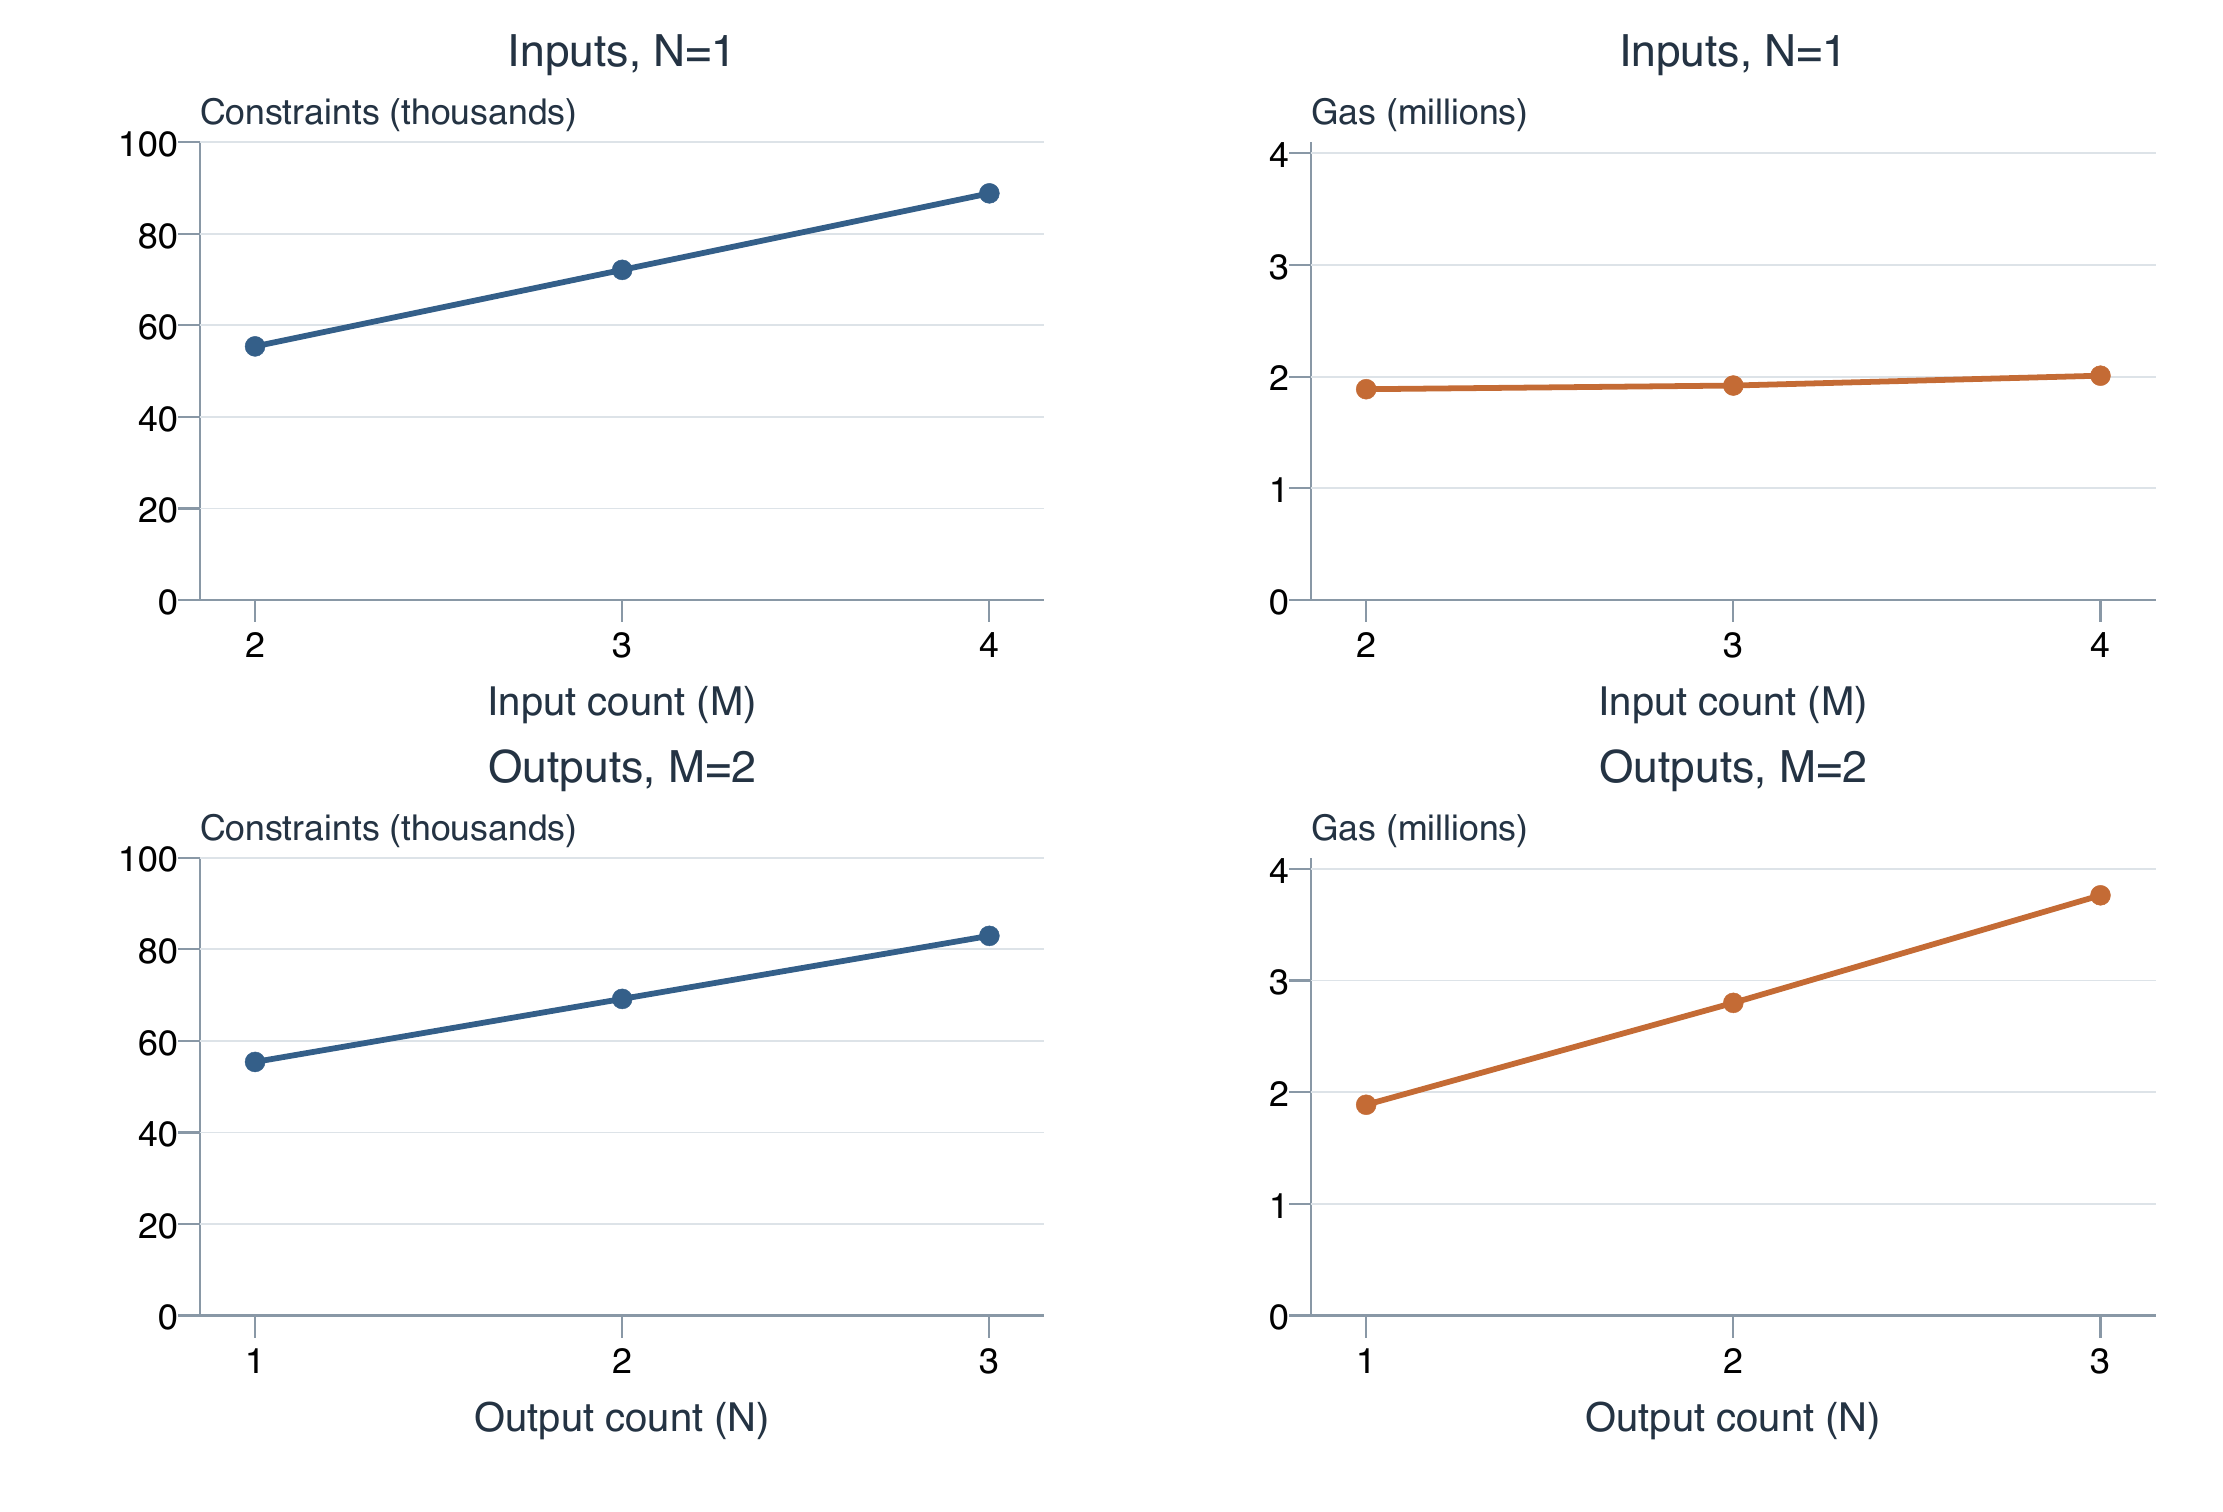
\includegraphics[width=.92\textwidth]{figures/evaluation/process.png}
\caption{Process costs when increasing inputs (top) or outputs (bottom). Matching metrics use the same vertical range; lines connect measured points.}
\label{fig:eval-process}
\end{figure*}

\paragraph{전달 방식과 공정 입출력의 영향.}
직접 전달은 송신 거래에서 수신자 회계 증표를 생성하고,
이전 증표 방식은 Transfer로 미해결 이전을 만든 뒤 Proceed로
수령을 완료한다. Table~\ref{tab:eval-transfer}은 직접 전달,
SharedSecret 변형과 정상 수령·회수 경로를 구분한다.

\begin{center}
\begin{minipage}{\columnwidth}
\centering\small\captionsetup{hypcap=false}
\captionof{table}{원료 전달 방식별 비용과 기능}
\label{tab:eval-transfer}
\begin{tabularx}{\columnwidth}{@{}p{20mm}rY@{}}
\toprule
방식 & gas & 기능 차이 \\ \midrule
직접 전달 & 2,366,228 & 감사 자료와 송신자 회수 기능 없음 \\
SharedSecret & 2,724,242 & 감사 자료 있음; 송신자가 후속 소비 식별 가능 \\
T $\to$ Proceed & 5,361,496 & 인수 전 회수 가능; 인수 뒤 소비는 직접 식별 불가 \\
T $\to$ Recall & 5,362,498 & 송신자가 인수 전에 회수 \\
\bottomrule
\end{tabularx}
\par\smallskip\begin{minipage}{\columnwidth}\footnotesize
T는 Transfer다. 직접 전달에는 감사 자료가 없고 다른 방식에는 있다.
기능 열은 설계상의 차이를, gas 열은 측정한 거래 비용을 나타낸다.
T $\to$ Proceed의 gas는 두 거래의 합이다. T $\to$ Recall은
보고된 경로 총합이며 두 거래의 합과 일치한다.
\end{minipage}
\end{minipage}
\end{center}


정상 수령의 합산 비용은
$3{,}577{,}414+1{,}784{,}082=5{,}361{,}496$ gas이다.
회수 경로의 5,362,498 gas는 Transfer와 Recall의 합이다.
정상 수령 합산값은 감사 없는 직접 전달의 약 2.266배다.
그러나 두 방식은 감사 기능의 유무도 다르고 거래 단계 수도 다르다.
따라서 이전 증표를 사용했기 때문에만 비용이 그만큼
늘었다고 해석할 수는 없다. 합산값은 연속 실행의 직접
측정값과도 구분한다.

이전 증표는 미해결 상태에서 기한·권한 조건을 만족하면 회수할 수
있으며, Proceed와 Recall이 같은 $rvnf$를 소비하므로 먼저
수락된 경로만 성공한다.
비교용 SharedSecret 직접 전달은 공유값 $o_{\rm shared}$를 이용한
$nf_{\rm shared}=H(cm,o_{\rm shared})$로 소비 식별자 계산 방식을 바꾼다.
송신자도 $cm,o_{\rm shared}$를 알면 수신자 회계 증표의 소비 거래를 식별할 수
있으나 소비 권한을 얻는 것은 아니다.
이 변형의 2,724,242 gas는 감사 없는 직접 전달보다
358,014 gas 크다. 감사 자료와 식별자 계산 방식이 함께 달라
감사 기능만의 비용으로 해석하지 않는다.

이전 증표의 공유 개방값으로 송신자가 계산하는 것은 $rvnf$이다.
인수 후 수신자 회계 증표의 $nf$는 수신자 소유 비밀에 의존하므로
그 개방값만으로 직접 계산할 수 없다. 이는 공개 시각·메타데이터를
이용한 모든 추론을 배제하는 성질은 아니다.
감사자는 Transfer에서 $rvnf$를 복원하여 Proceed를 찾고,
그 기록에서 수신자 회계 증표의 미래 $nf$를 복원한다.
잔여 회계 증표도 별도의 미래 식별자를 통해 추적한다.

공정 규모는 출력 $N=1$에서 입력 $M$을 2, 3, 4로,
입력 $M=2$에서 출력 $N$을 1, 2, 3으로 바꾸어 평가하였다.
입력 상태 합 $(320,30,231)$과 출력 상태 합 $(300,30,261)$을
고정하였다. 이 조건은 시제품의 세 상태 성분에 대한 것으로
모든 산업 공정을 대표하지 않는다.

\begin{table}[t]
\centering\small
\caption{Process cost by input and output count}
\label{tab:eval-process}
\begin{tabular*}{\columnwidth}{@{\extracolsep{\fill}}lrrrr@{}}
\toprule
Sweep & $M$ & $N$ & Constraints & Gas \\ \midrule
Inputs & 2 & 1 & 55,402 & 1,887,935 \\
Inputs & 3 & 1 & 72,116 & 1,920,611 \\
Inputs & 4 & 1 & 88,832 & 2,009,039 \\
Outputs & 2 & 1 & 55,402 & 1,887,935 \\
Outputs & 2 & 2 & 69,172 & 2,800,596 \\
Outputs & 2 & 3 & 82,944 & 3,763,779 \\
\bottomrule
\end{tabular*}
\par\smallskip\begin{minipage}{\columnwidth}\footnotesize Input sum $(320,30,231)$ and output sum $(300,30,261)$ are fixed. The $2\to1$ baseline differs by 21,318 gas from Table~\ref{tab:eval-events}; the cause is unresolved.\end{minipage}
\end{table}


Table~\ref{tab:eval-process}에서 입력을 2개에서 4개로 늘리면
제약 수는 60.34\%, gas는 6.41\% 증가하였다. 출력을 1개에서
3개로 늘리면 각각 49.71\%와 99.36\% 증가하였다.
이 구간에서는 출력 증가가 입력 증가보다 gas에 더 큰 변화를
동반하였다. 입력이 늘면 기존 기록을 검사하는 일이 추가되고,
출력이 늘면 새 기록을 등록하는 일이 추가된다.
관측값은 이 차이와 부합하지만, 어느 연산이 얼마를 차지하는지는
비용을 더 나누어 측정해야 알 수 있다.
이 실험의 $M=2,N=1$ gas는 1,887,935로 기본 거래의
1,866,617과 21,318 차이가 난다. 증가율은 공정 규모 실험
안의 기준값으로 계산하며, 두 실행의 차이는 미확인으로 남긴다.

\subsection{기존 연구와의 비교}

\begin{table}[t]
\centering\small
\caption{Published and measured transaction gas}
\label{tab:eval-published}
\begin{tabularx}{\columnwidth}{@{}>{\raggedright\arraybackslash}p{24mm}rY@{}}
\toprule
System or path & Gas & Scope \\ \midrule
Azeroth zkTransfer~\cite{jeong-azeroth-2023} & 1,555,957 & Published; change in ENA \\
Direct baseline & 2,366,228 & No audit; change Note \\
SharedSecret direct & 2,724,242 & Audit; shared spend identifier \\
zkDPP Transfer & 3,577,414 & Audit; Voucher and change Note \\
zkDPP Transfer $\to$ Proceed & 5,361,496 & Normal receipt; two-event sum \\
\bottomrule
\end{tabularx}
\par\smallskip\begin{minipage}{\columnwidth}\footnotesize Azeroth: Groth16, MiMC7, depth 32. Remaining rows: this evaluation. Different settings and functionality preclude an efficiency ranking.\end{minipage}
\end{table}


Table~\ref{tab:related}의 기능 비교를 바탕으로,
평가에서는 추적·차단의 작업 단위와 거래 비용을 비교한다.
Sahai 등의 공급망 전이와 Babel 등의 자격증명·토큰 연결은
응용 측면의 기준선이며, GGM의 후속 출력 추적, Azeroth의
거래 결합 감사 정보와 CAP의 정책별 열람·동결은 감사·집행의
선행 구성이다. zkDPP의 기능 검증은 이를 회계 전이,
제품 주장·종료의 구분, 미소비 회계 증표·미해결 이전 증표의
차단으로 연결한 대표 경로를 확인한다. 같은 응용 관계와 신뢰
조건을 갖는 구성보다 우수하다는 결론은 이 검증에서 도출하지 않는다.

Azeroth는 Groth16, MiMC7, 깊이 32의 설정에서
zkTransfer의 비용을 1,555,957 gas로 보고한다~\cite{jeong-azeroth-2023}.
Table~\ref{tab:eval-published}은 이 값과 본 평가의 전달 비용을
작업 범위와 함께 제시한다. Azeroth는 암호화 계정(ENA)과
머클 노트를 함께 사용하여 잔여 금액을 ENA에 반영하고,
본 평가의 직접 전달 기준선은 잔여분을 새 회계 증표로 등록한다.
증명계·검증기·해시·원장 조건도 같지 않다.
이 표는 각 전달 방식에서 무엇을 하나의 작업으로 측정했는지
보여 주며, gas 차이를 잔여분 처리 방식 하나의 효과로 분리하지는 못한다.
자체 직접 전달은 Azeroth를 같은 환경에서 재현한 결과가 아니다.

Sahai의 Hyperledger Fabric 구현은 EVM gas와 다른 지표를
사용한다~\cite{sahai-supply-chain-2020}.
Babel 등의 측정은 분산 원장을 사용하지 않는 운영자 원장을
대상으로 하므로 그 연산 시간을 거래 영수증 확인까지 포함한
E2E와 직접 비교할 수 없다~\cite{babel-hicss-2025}.
CAP의 동결도 레코드의 소비·재발행으로 이루어져 현재 상태를
변경하는 zkDPP와 작업 구성이 다르다~\cite{espresso-cap-spec-2022}.
따라서 본 평가는 대표 기능의 연결과 기능별 비용·규모 변화를
제시하며, 외부 시스템과의 효율성 순위를 정하지 않는다.
% Flush evaluation floats; restore the full text height after double-column floats.
\clearpage
\makeatletter
\global\@colht\textheight
\global\@colroom\textheight
\global\vsize\textheight
\makeatother

% Normative source: sections 1.2, 2, 3.5, 9, 10, 13--17.
\section{논의와 한계}
\label{sec:limits}

이 절은 앞의 검증·추적·차단 결과가 무엇을 뜻하는지,
그 결과를 실제 운영에 적용하려면 무엇이 더 필요한지 구분한다.

\subsection{회계 값의 해석}

zkDPP는 원장이 수락한 값과 디지털 전이가 정해진 규칙을 따르는지
검증한다. 최초 증빙의 진실성, 실제 공정·재료·제품과 문서의 대응은
등록 승인자나 외부 검사에 달려 있다. 탄소 값도 수용한 초기 값과
운송·공정 증분의 배분 결과이지, 전체 생애주기의 측정값이 아니다.
초기 탄소를 0으로 둔 경우와 폐기물의 $a=e=0$도 실제 배출이
없었다는 뜻은 아니다. 공개 DPP 검증은 지정한 필드와 발급 기록의
일치를 확인하며 문서 전체나 규제 준수를 인증하지 않는다.

합계가 맞아도 제품별 탄소 배분이 실제 배출량을 뜻하는 것은 아니다.
식~\eqref{eq:process-carbon}은 질량 0 출력에 탄소를 배분하지 않고
정수 잔여를 양의 질량 출력에 준다. 예를 들어 탄소 합계가 1인 입력을
질량 $(0,1,1)$의 세 일반용 출력으로 나누면 탄소는 $(0,1,0)$이다.
이는 정해진 정수 회계 규칙을 따른 결과일 뿐, 두 제품의 실제
탄소발자국을 측정한 결과는 아니다. 최초 탄소 값과 공정 증분의
진실성, 제품별 배분 기준의 적절성은 여전히 외부 검증이 필요하다.
\ref{sec:model-validation}절에서는 질량 0 출력에 잔여를 주려는
이전 사례를 현행 규칙이 거부하는지 검사한다.

\subsection{감사·차단의 범위}

후속 추적은 도달한 거래의 모든 출력을 포함하는 디지털 의존관계
정책이다. 실제 오염 범위나 피해 정도를 판정하지 않으며, 시작점과
차단 승인도 신뢰된 감사자의 판단이다. 원장의 동결은 현재 미소비
Note와 미해결 Voucher의 다음 사용을 거부한다. 이미 소비한 기록을
되돌리거나 발급된 Claim을 취소하거나 물리적 유통을 막지는 못한다.
감사 중 새 파생 객체가 생기면 새 시점에서 다시 조사해야 한다.

zkDPP는 부모 참조와 출력의 미래 식별자를 한 목록에 묶어 암호화해
기록마다 바로 찾도록 한다. 다른 방법도 있다. 관련 출력과 복호화 키를 모두
모아 소비 식별자에서 출력의 종류·위치를 찾는 조회표를 만들면
부모 참조를 기록에 암호화해 두지 않아도 선행 객체를 찾을 수 있다.
단, 자료의 누락·중복을
검사해야 하며, 미소비 객체를 소유자 협력 없이 차단하려면 미래
식별자를 얻는 별도 수단도 필요하다. 직접 기록과 전체 조회표 중
어느 쪽의 비용이 낮은지는 여기서 측정하지 않았다.

\subsection{구현과 평가의 한계}
\label{sec:implementation-limits}

일반 Process 설계와 확인한 구현의 범위는 다르다.
소스로 확인한 고정 구현은 입력 3개를 일반용·폐기물 출력 하나씩으로
바꾸는 특정 정책이며, 일반용 출력의 질량은 양수여야 한다.
폐기물 출력에는 질량 0을 허용한다. 입출력 수를 바꾸는 실험용 회로는
별도 코드이며 모든 출력을 양의 질량인 일반용으로 제한한다.
따라서 이들 구현이 일반 설계의 여러 일반용 출력에 대한 질량 0
배분 규칙까지 구현한 것은 아니다~\cite{zkdpp-implementation-profile-2026}.
이 소스 확인과 앞 절의 성능 보고값을 같은 실행 결과로 간주하지 않는다.

첫째, 세 보안 성질의 암호 가정이 실제 증명계·군·해시와 인코딩에서
성립하는지, 감사키의 생성·분산·복원과 조각 전달이 올바른지 확인해야 한다.
정리 3은 공개 조각 확인 자료와 K개 미만 조각을 포함하지만,
DDH·독립 무작위 오라클·다중 정리 영지식을 전제로 한다.
참여자 부패나 능동 질의까지 다루는 결과는 아니다.

둘째, 인용한 보존 기능 시험의 대표 실행을 넘어 현행
회로·계약·클라이언트를 같은 경로에서 시험해야 한다.
아홉 거래의 정상·거부 사례, 생성 때 남긴 식별자와 실제 소비의
일치, 분기·합류·자료 누락의 추적, 전체 대상의 부분 실패·경합과
공통 시점 완료 판정을 함께 확인해야 한다.

셋째, 측정 코드·설정과 원시 결과를 연결해 독립 실행의 시간 변동을
확인해야 한다. 키 복원의 1,000회 내부 평균은 독립 반복이 아니다.
Process의 기준값 사이 21,318 gas 차이 역시 설명되지 않았다.
외부 시스템의 성능 순위를 정하려면 작업 단위와 환경을 맞춰야 한다.

\section{결론}
\label{sec:conclusion}

본 논문은 공급망 자료를 숨긴 채 회계 규칙을 검증하고,
근거에 문제가 생기면 관련 기록의 다음 사용을 막는 zkDPP의
구성과 보장 조건을 제시하였다.
거래마다 실제 입력과 출력의 미래 소비 식별자를 암호화해 남긴다.
거래 증명은 이 자료가 실제 계산과 맞는지도 검사한다.
승인된 감사자는 암호문을 열어 이력을 따라가고,
아직 소비되지 않은 관련 기록 전체를 차단한다.
회계 증표의 소유자 생성과 별도 이전 증표를 통해 미래 식별자를
생성 때 남기고, 같은 이력을 비공개 검증과 사후 집행에 사용한다.

보안 분석은 정상 요청이 기대한 결과를 내는 정확성,
틀린 거래·추적·완료 보고를 받아들이지 않는 건전성,
공개 자료에서 숨긴 내용을 구별하기 어렵게 하는 프라이버시로
구성하였다. 이 결과에는 명시한 암호·원장·권한 가정이 필요하다.
프라이버시는 무작위 오라클 모형에서 참여자의 비밀·개방값이
공개되지 않은 정상 이력을 읽는 수동 외부 관찰자에 한정한다.

차단에서는 대상 전체를 하나의 공통 시점에 확인해야 한다.
각 대상의 동결 성공 기록이 있어도 모두가 동시에 차단된 적은
없을 수 있다. 또 조사한 뒤 다른 거래가 대상을 먼저 소비할 수 있다.
zkDPP는 이런 대상을 목록에서 지우지 않고 미완료 사유로 남긴다.
전체 대상이 미소비·차단 상태임을 확인하고 그 상태가 유지되는 동안에만
그 대상을 통한 후속 사용을 거부한다.

기호 모델에서는 네 사례군의 334개 추적 결과를 독립 계산과 대조했다.
두 계산은 일치했지만 기록에서 시작하는 규칙이 명세와 다른 부분이
있으므로 명세 전체를 검증한 결과는 아니다.
누락 자료, 부분 동결과 소비 경합도 검사하였다.
질량이 0인 출력에 탄소 잔여가 몰리는 사례는 계산식의 합계가
맞아도 최종 제품군의 탄소 배분까지 보장되지는 않음을 보여 주었다.

시제품에서는 분기 이력의 추적·동결·결과 확인을 연결한 대표 실행과
아홉 거래의 비용을 제시했다. 감사 기능은 측정 조건에서
제약 수를 31.70--202.93\%, gas를 9.69--54.67\% 증가시켰다.
Transfer에서는 암호 계산의 스칼라 곱셈과 감사 자료 저장이
각각 추가 회로 비용과 추가 gas의 큰 부분을 차지했다.
기록 1,000개의 후속 추적은 9.760초,
대상 1,000개를 개별 거래로 동결하는 데에는 60.540초가 걸렸다.
두 시간은 서로 다른 작업을 따로 측정한 값이다.
공정 입출력 수를 바꾼 구간에서는 출력 증가가 입력 증가보다
gas에 더 큰 변화를 동반하였다.

제시한 보장은 승인된 회계 정책에 따른 디지털 기록과 그 후속 사용에
관한 것이다. 입력 증빙의 진실성, 이미 발급된 제품 주장의 취소와
물리적 회수는 외부 절차의 영역이다.
후속 과제는 현행 암호 구성의 가정 충족과 전체 통합 실행을 확인하고,
측정 판본의 대응 및 독립 반복 통계를 확보하는 것이다.

\begingroup
\referencefont
\small
\raggedright
\bibliographystyle{unsrt}
\bibliography{references}
\endgroup
\clearpage
\appendix
\renewcommand{\thesection}{\Alph{section}}
\renewcommand{\thesubsection}{\Alph{section}.\arabic{subsection}}
\setcounter{equation}{0}
\renewcommand{\theequation}{A.\arabic{equation}}
\section{데이터 형식과 세부 실행 규칙}
\label{app:protocol-details}

이 부록은 \ref{sec:system}–\ref{sec:audit}절의 운영 가정과
사용하는 값의 정확한 표현, 실행 조건을 정리한다.

\subsection{참여 주체와 감사키}
\label{app:system-model}
\label{app:audit-key}

등록 승인자는 최초 값과 동일 물량의 중복 등록 여부를 판단하고,
정책 관리자는 가공·발급 조건과 검증키, 기업의 가공 권한을 등록한다.
이 두 역할의 판단·등록과 감사자의 조사 시작점 선택·상태 집행을 신뢰한다.
감사자와 상태 관리자는 같은 주체이며, 감사 클라이언트는 그 주체의
소프트웨어로 별도의 신뢰 주체가 아니다.

원장은 확정 순서·변경되지 않는 수락 기록·인증된 상태 읽기와
원자적 거래를 제공한다고 가정한다. 원격 조회 결과도 인증해야 한다.
질량·재활용 크레딧·탄소와 운송·공정 증분은 외부에서 제공되며,
실제 측정·공정 수행과 제품·문서의 대응은 외부 확인에 의존한다.

송신자는 이전 증표의 개방값을 보관하고, 이전 거래 제출 전이나 함께
인증된 비밀 채널로 수신자에게 전달한다.

감사 자료는 공개키 $PK_B$로 암호화하고 비밀키 $SK_B$로 읽는다.
본문의 표기 $pk_{\mathsf{audit}}=PK_B$,
$sk_{\mathsf{audit}}=SK_B$도 같은 키를 뜻한다.
$SK_B$는 Shamir 방식으로 $N$개 비밀 조각에 분산하며,
서로 다른 $K$개 조각으로 복원한다($1\leq K\leq N$).
위원들은 조각을 하나씩 보관한다.~\cite{shamir-secret-sharing-1979}
초기 설정자는 원본 키 사본을 남기지 않고 조각을 각 위원에게
비밀로 전달한다고 가정한다.

외부 승인 뒤 서로 다른 $K$명의 위원이 인증된 비밀 경로로 조각을 전달하면,
감사자는 구성원·배포·키 식별과 공개 확인 자료를 검사하여 $SK_B$를 복원한다.
복원한 키에서 계산한 공개키가 배포된 $PK_B$와 같은지도 확인한다.
감사 승인과 조각 전달은 신뢰된 외부 절차로 수행한다.

유효 키를 복원한 감사자는 원장 기록과 형식을 확인한 뒤
암호문 $ct$를 로컬에서 다음과 같이 복호화한다.
\begin{equation}
 M\leftarrow\mathsf{AuditDec}(sk_{\mathsf{audit}},ct)
 \label{eq:decrypt}
\end{equation}
키 식별·형식·복호화가 맞지 않으면 오류로 처리하고,
$SK_B$와 위원 조각은 공개 거래나 감사 결과에 넣지 않는다.
위원회는 키 복원에 협력하며 기록마다 다시 참여하지 않는다.

배포마다 키 하나를 사용하며, 복원한 키의 열람 범위는 그 키로
암호화한 기록 전체다. 시작점·시점은 업무상 조사 범위를 정한다.
비인가 관측자의 키·조각 보유 조건과 세 보안 성질은
\ref{sec:analysis}절과 부록~\ref{app:security-details}에서 정의한다.

\subsection{개방값·식별자·정수 범위}
\label{app:formats}

해시 입력은 타입과 필드 경계를 보존하는 정규 직렬화를 사용한다.
$H_{\mathsf{tag}}$는 \texttt{zkDPP:tag:v2} 도메인의 해시이며,
\texttt{Note}, \texttt{Voucher}, \texttt{Nullifier} 등 목적을 구분한다.
개방 난수·소유 비밀의 유효 영역, 문자열 정규화와 유한체로의 해시
변환은 배포 설정에서 고정한다.

회계 증표와 이전 증표의 개방값·커미트먼트는 다음과 같다.
\begin{align}
 n&=(d,\rho,q,a,e,o,\omega_N),\nonumber\\
 cm&=H_{\mathsf{Note}}(d,\rho,q,a,e,o,\omega_N)
 \label{eq:note}
\end{align}
\begin{align}
 v&=(d,\rho,q,a,e,o_S,o_R,D,\omega_V),\nonumber\\
 rv&=H_{\mathsf{Voucher}}(d,\rho,q,a,e,o_S,o_R,D,\omega_V).
 \label{eq:voucher}
\end{align}
$d,\rho,q,a,e$는 문서·역할·회계 값이고,
$o,o_S,o_R$는 소유자·송신자·수신자다.
$\omega_N,\omega_V$는 비밀 개방 난수, $D$는 절대 회수 기한이다.
회계 증표의 소비 식별자는 식~\eqref{eq:nf}로,
이전 증표의 공통 해결 식별자는 다음과 같이 계산한다.
\begin{align}
 s_{\mathrm{res}}&=H_{\mathsf{VoucherResolutionSecret}}(\omega_V),\nonumber\\
 rvnf&=H_{\mathsf{VoucherNullifier}}(rv,s_{\mathrm{res}})
 \label{eq:rvnf}
\end{align}
인수와 회수는 각자의 소유권 지식을 증명하지만 동일한 $rvnf$를 쓴다.

문서 해시는 다음 세 필드에 한정한다.
\begin{equation}
 \mathsf{DocumentInfo}=(\mathit{ProductName},\mathit{LotID},\mathit{Unit})
 \label{eq:doc}
\end{equation}
$d=\mathsf{HashDocumentInfo}(\mathsf{DocumentInfo})$이며,
지정 DPP 경로에서 추출한 필드의 누락·잘못된 타입·모호한 인코딩은 거부한다.
객체 조회 키는 \texttt{ObjectRef} 도메인에 타입과 원시 참조를 함께
결합한다. 소비·상태 조회의 $nf,rvnf$도 타입별로 구분한다.
Claim은 등록 여부만 두며 포함 관계 트리·미래 식별자·상태가 없다.

모든 회계 값과 중간 합·곱·나머지는 지정된 정수 범위에 있어야 한다.
유한체에서 값이 돌아오는 계산을 정수 등식으로 오인하지 않도록
범위를 함께 검사한다. 재활용 크레딧의 바닥 함수 배분은
다음 몫·나머지 조건으로 확인한다.
\begin{equation}
 \begin{gathered}
 y=\left\lfloor\frac{xq}{Q}\right\rfloor,\qquad Q>0,\\
 xq=Qy+r,\qquad 0\leq r<Q.
 \end{gathered}
 \label{eq:floor}
\end{equation}
탄소의 비례 배분은 정확히 나누어떨어진다는 가정 아래
$r=0$, 따라서 $xq=Qy$로 표현한다.
분모 0은 허용하지 않는다. 비교식의 단위와 고정 배율도 일치해야 한다.

소비 식별자의 불변성은 효율적인 실행에서 얻은 같은 타입 참조의
개방 증인 $w,w'$에 대해
$\mathsf{SpendId}(w)=\mathsf{SpendId}(w')$이며
생성 시 암호화한 값과도 같다는 조건이다.
이 조건은 개방값의 결합성과 소유자 해시의 충돌 저항성 아래 성립한다.
$\mathsf{OwnerKey}(s)=H_{\mathsf{Owner}}(s)$는 정규 비밀값에
소유자용 해시를 적용한다. 생성·소비 때 소유자 표시가 같은데
서로 다른 비밀을 사용했다면 소유자 해시의 충돌 쌍을 얻는다.
그 사건 밖에서는 두 비밀과 소비 식별자가 같다.
충돌 상계와 전체 논증은 부록~\ref{app:soundness-details}에 둔다.

\subsection{설정과 거래 수락}
\label{app:acceptance}

거래 종류 $k$의 공개 문장은
$x=(u,\boldsymbol\nu,\boldsymbol r,ct)$이고,
비공개 증인은
$w=(\boldsymbol z,\boldsymbol{sk},\boldsymbol{path},\eta)$다.
$u$는 배포·원장·이벤트 경로·정책·권한·루트·기한 등 공개 메타데이터,
$\boldsymbol z$는 실제 입출력 개방값이다.

감사 공개키 $PK_B$는 회로의 고정값이다.
키 식별과 회로·검증기의 대응은 배포 설정에서 정한다.
감사키의 분산·복원은 부록~\ref{app:audit-key}의 절차를 따른다.
이벤트 증인에 $SK_B$나 위원회 비밀 조각을 요구하지 않는다.

부모의 원시 참조 $P_i$와 소비 가능한 출력의 미래
식별자 $\nu_i^{\rm out}$를 한 목록으로 만든다.
$cm,rv$는 정규 유한체 원소이며 타입은 거래 관계로 정한다.
부모가 $m$개이고 소비 가능한 출력이 $s$개이면
\begin{equation}
 M=(P_0,\ldots,P_{m-1},\nu_0^{\rm out},\ldots,\nu_{s-1}^{\rm out}).
 \label{eq:audit-vector}
\end{equation}
이 목록은 실제 입출력 개방값에서 계산한 $M(w)$다.
암호문 $ct=(R,\boldsymbol C)$는 하나의 난수 $0<\eta<\ell$로 만든다.
$\ell$은 생성점 $G$의 위수이며, 아래 덧셈·뺄셈은 평문 유한체에서 한다.
\begin{equation}
 \begin{aligned}
 R&=\eta G,\qquad Z=\eta PK_B,\\
 \kappa&=H_{\mathsf{AuditKey}}(Z_x,Z_y),\\
 C_j&=M_j+H_{\mathsf{AuditMask}}(\kappa,j).
 \end{aligned}
 \label{eq:audit-vector-encryption}
\end{equation}
인덱스 $j$는 전체 목록에서 0부터 시작한다. 저장할 때는 부모의
암호화 값 $m$개와 미래 식별자의 암호화 값 $s$개를 두 배열로
나누지만, 같은 $R$을 쓰는 한 암호문이다. 감사자는 두 배열을 다시
이어 붙이고 $Z=SK_B R$로 같은 $\kappa$를 계산해 각 마스크를 뺀다.
미래 식별자 배열에서도 인덱스를 0으로 다시 시작하지 않는다.

Transfer의 출력 순서는 이전 증표·잔여 회계 증표이고,
평문 목록은 $(cm_{\rm in},rvnf_T,nf_C)$다.
Claim에는 미래 식별자가 없고, Exit·Issue는 부모만 암호화한다.
Entry는 부모 없이 출력 Note의 미래 식별자만 암호화한다.
따라서 아홉 거래 모두 암호화할 값이 적어도 하나 있다.

키 유도 입력은 식~\eqref{eq:audit-vector-encryption}의 점 좌표이며,
거래 문맥·목록 길이·타입은 회로의 정해진 형상과 전체 공개 문장으로 결합한다.
계약은 공개 입출력 뒤에 $R$의 좌표·두 암호화 배열을 같은 순서로
붙여 증명을 검증하고, 검증한 자료를 그대로 기록해야 한다.
회로는 난수의 범위와 비영 값을 검사하며, 거래 사이의 독립 난수
생성은 클라이언트의 책임이다. 동일 키에서 난수를 재사용하면
같은 위치의 마스크가 반복되어 평문 간 차이가 드러날 수 있다.
복호화 정확성은 이 관계의 모든 허용 난수에서 $M(w)$가 복원된다는
조건이다.

공통 암호·생애주기 관계와 선택한 회계 관계를 합쳐 검사한다.
\begin{equation}
 \mathcal{R}_k=\mathcal{R}^{\mathrm{core}}_k
                  \land\mathcal{R}^{\mathrm{acct}}_k
 \label{eq:relation}
\end{equation}
공통 관계에는 개방·소유권·포함 관계·소비 식별자·정수 범위,
중복 금지와 출력·감사 결합을 포함한다.
고정 경로는 이벤트별 검증기 선택으로 종류를 결합하고,
등록 경로는 정책 $p$와 필요한 적용 범위를 증명에 결합한다.

배포자는 암호·직렬화·거래 형상·역할·위원회와 고정 검증기를 설치한다.
회계·이전 증표는 별도의 깊이 32 추가 전용 머클 트리에 저장하며,
초기 트리는 비어 있고 그 루트는 수락된 루트다.
노드·리프 수·현재 및 과거 수락 루트를 보관해 포함 경로를
공개 자료로 재구성할 수 있게 한다. 용량 초과는 거래 전체를 거부한다.
소비·생성 색인, Claim과 감사 기록도 빈 상태에서 시작하고
$\aid$는 1부터 증가한다.

등록 정책의 식별자는 거래 종류 $k$, 등록 주체 $a$, 그 주체의
정책 번호 $b$와 버전 $v$로 계산한다.
\begin{equation}
 p=H_{\mathsf{PolicyRef}}(k,a,b,v).
 \label{eq:policy-ref}
\end{equation}
원장은 권한 있는 등록 주체에 $a$를 부여하고 정책 번호·버전을
예약한 뒤, 그 식별자에 검증기와 정확한 입출력 수를 한 번 등록한다.
입출력 수는 불변 등록 정보와 회로에서 고정하며,
거래 때 두 형식이 일치하는지 검사한다.
관계 명세와 회로·검증키의 대응을 공개하고,
가공의 각 $(m,n)$ 형태는 별도 정책 버전 또는 번호와 검증키를 쓴다.
계산 규칙·형상·검증키를 바꿀 때는 새 식별자를 등록한다.
검증기 메타데이터는 불변이고 정책 활성값은 참에서 거짓으로만 바뀐다.
비활성화는 이후 제출에 적용하며 과거 수락·Claim을 취소하지 않는다.
가공의 불투명 식별자 \texttt{scope}에 대해 제출자 또는 자격증명의
범위 권한과 $(scope,p)$ 사용 권한을 함께 검사한다.
소유권 지식만으로 모든 정책을 사용할 수는 없다.
고정 이벤트의 정책 표식 0은 등록 정책 식별자와 구분한다.

증명자는 실제 개방값·포함 경로를 준비하고,
입력 소비 식별자, 출력 참조·미래 식별자와 감사 암호문을 계산하여
전체 관계의 증명을 만든다. 원장은 경로·형상·정책·권한,
수락 루트·현재 미소비·활성·실행 시 기한과 모든 출력 키의 신규성을 검사한다.
같은 거래 안의 실제 입력 참조, 타입별 소비 식별자와 출력 조회 키도
각각 중복될 수 없다. 이미 등록된 Claim의 재생성도 거부한다.
통과하면 한 트랜잭션에서 $\aid$ 배정, 소비 기록,
트리 추가 또는 Claim 등록, 감사 기록과 모든 출력의 생성 색인을
갱신하고 다음 $\aid$로 진행한다. 실패하면 모두 취소한다.
수락된 소비·생성·감사 기록은 불변이다.

상태는 별도 트리가 아닌 타입별 미래 소비 식별자의 매핑으로 관리한다.
기본값은 Active, Revoked는 종단이며 Active에서 바로 갈 수 없다.
감사자는 실제 생성 기록을 확인하여 해당 객체의 미래 소비 식별자를 선택한다.

Entry는 유효한 명시 초기 탄소 $e_0$를 보존한다.
생략만 클라이언트에서 0으로 정규화하며 잘못된 명시 값을 0으로 바꾸지 않는다.
그 값은 개방값·증인에 결합되고, 기본값을 회로의 $e_0=0$ 제약으로
해석하지 않는다. Transfer의 $D$는 증표 안의 값과 같고,
생성 실행 시 현재보다 미래이면서 배포의 허용 범위 안에 있어야 한다.
Recall은 실행 에포크가 $D$인 경우도 허용하고 이후 제출은 거부한다.

\subsection{추적 규칙}
\label{app:trace-details}

실제 그래프는 수락 때의 실제 생성·소비 값으로 정의한다.
객체에서 그것을 소비한 이벤트로, 이벤트에서 전체 출력으로 간선을 잇는다.
생성이 소비보다 앞서므로 순환이 없다.
인증 조회는 고정 $H_t$의 실제 값 또는 오류를 반환하며,
확정되지 않은 블록 번호만으로 확정성을 판단하지 않는다.

선행 객체 시작은 그 객체·생성 이벤트·둘 사이 간선을 포함한다.
선행 기록 시작은 지정 이벤트와 모든 직접 출력·출력 간선을 포함한 뒤
실제 부모를 거슬러 올라간다. 따라서 출력 없는 Exit도 시작점이 된다.
재귀 중에는 부모의 생성 기록을 읽되 그 기록의 다른 출력은 추가하지 않는다.
각 부모의 타입·수·순서·중복과 더 이른 생성 순서를 확인한다.
부모가 비어 있으면 Entry여야 하며 초기 등록 집합에 기록한다.

후속 객체 시작은 그 객체 하나, 기록 시작은 그 기록의 전체 출력을
초기 큐에 넣는다. 시작 기록 자체와 출력 간선을 출발점이라는 이유로
추가하지 않으며, 출력 없는 기록의 후속 결과는 빈 결과다.
이는 종료 이전의 선행 조사와 다르다.
미소비 Note/Voucher는 타입 참조·미래 식별자와 함께 각각 $F_N,F_V$에,
도달 Claim과 Exit는 별도의 종단 집합에 기록한다.

객체의 존재·생성 기록·출력 위치·이벤트 형상과 공개 트랜잭션 자료를
확인하고 전체 벡터를 복호화한 뒤 정해진 위치에서 필요한 값을 얻는다.
소비 식별자 조회가 양수이면 해당 기록이 실제 생성보다 나중이고,
공개 입력에 같은 타입의 식별자가 있는지 확인한다.
소비 이벤트의 부모 목록에 현재 객체가 포함됐는지도 검사한다.
함께 복호화한 다른 부모를 후속 그래프의 선행 경로로 추가하지 않는다.
부모와 소비 식별자의 실제 입력 결합은 수락 증명에 의존한다.

같은 이벤트의 복호화·출력 확장은 한 번만 수행할 수 있지만,
재방문에서 새로 도달한 객체와 입력·출력 간선은 보존한다.
같은 생성 기록을 읽는 것과 그 기록의 모든 출력을 후속으로
추적하는 것은 다른 처리다.
동일 객체의 상충하는 식별자, 서로 다른 객체의 같은 타입 식별자는
중복으로 합치지 않고 오류로 처리한다.
숫자가 같아도 타입이 다른 객체·식별자는 구분한다.

키·자료 부재나 발견된 디코딩·복호화·일관성 오류는 실패다.
부분 진단 자료를 반환할 수 있어도 완성된 그래프나 전체 대상으로
보고할 수 없다. 승인 부재·잘못된 원장 문맥은 집행 전에 거부한다.

\subsection{감사·차단의 집행과 반환}
\label{app:freeze-execution}

\ref{sec:audit}절의 절차는 추적·일관성 검사를 마친 뒤 동결을 시작한다.
검사가 실패하면 \Alg{TRACE\_FAILED}로 종료하고 이 실행의 동결 거래는
제출하지 않는다. 추적이 성공하면 전체 미소비 집합을 $T$로 고정하며,
비어 있으면 \Alg{NO\_LIVE\_TARGETS}를 반환한다.

대상별 처리는 Table~\ref{tab:freeze}를 따른다.
한 대상의 실패가 이미 성공한 동결을 되돌리지는 않는다.
가능한 다른 대상은 계속 처리하되 시도·확인은 유한 한도 안에서 끝낸다.
미시도·실패·불명확한 제출은 사유와 함께 남긴다.
\begin{table}[htbp]
\centering\small
\caption{Per-target action at execution time}
\label{tab:freeze}
\begin{tabularx}{\columnwidth}{@{}YY@{}}
\toprule
Observed state & Action in this run \\
\midrule
Unspent, Active & Submit a typed Freeze transaction \\
Unspent, Frozen/Revoked & Record an existing block \\
Already spent & Retain target and consumer as a race \\
Read failure & Retain target as unconfirmed \\
\bottomrule
\end{tabularx}
\end{table}

거래 영수증은 제출 결과의 근거이고 최종 차단 여부는 공통 $H_r$에서 판단한다.
동결 제출이 다른 실행의 선행 동결 때문에 거부됐더라도,
공통 시점에서 이미 차단됐음이 확인될 수 있다.
먼저 소비된 사실을 관찰했다면 그 소비 이전의 시점을 골라 완료로
보고할 수 없다. 결과에는 시작점, $H_t$, 추적 결과, 전체 $T$,
대상별 시도·영수증·상태, 공통 $H_r$ 또는 그 부재와 최종 판정을 남긴다.
정상 추적과 비어 있지 않은 $T$를 얻은 실행은 \ref{sec:audit}절의
세 완료 조건을 모두 만족하면 \Alg{COMPLETE\_AT\_CHECKPOINT}를,
그 밖에는 전체 대상을 보존한 \Alg{INCOMPLETE}를 반환한다.

\section{조건부 보안 증명의 세부사항}
\label{app:security-details}

이 부록은 VI절의 세 정리에 사용한 실험과 암호 가정을 명시한다.
모든 공격자와 실행·객체·증명·질의 수는 보안 매개변수 $\lambda$의
다항식으로 제한한다. 확률은 명시한 전체 실행에 관한 것이다.
원장의 권한·인증·확정·현재 상태 집행과 신뢰된 감사자의 동작은
모델 전제이며 아래 암호 가정으로 새로 증명하지 않는다.

\subsection{정확성 증명}
\label{app:correctness-details}

정확성 게임은 정직한 생성에 사용한 증인을 보관한다.
거래는 전체 증명 관계와 실행 조건, 출력 신규성과 트리 용량을
만족하며 그 조건이 실행까지 유지되어야 한다.
공개 DPP 검증은 발급이 포함된 확정 이력과 그 발급에 맞는 정규 문서를 쓴다.
추적은 유효 시작점·확정 $H_t$·유효 감사키를 사용하고,
필요한 유한 기록과 종료하는 인증 조회가 있어야 한다.
고정 $H_t$의 조회에는 그 이후 원장 전체의 무경합을 요구하지 않는다.

차단 승인이 있고 정확한 전체 $T$가 비어 있지 않다면,
$H_t$부터 $H_r$까지 대상 소비와 차단 해제가 없어야 한다.
Active 대상의 합법적 동결, 모든 제출 결과·조회,
사용한 관찰을 반영하는 같은 확정 이력의 $H_r$을 정한 유한 한도
안에서 확보해야 한다. $T=\varnothing$에는 이 추가 조건 없이
빈 대상 분기를 적용한다.

위 조건이 성립하는 요청에서 기대한 결과를 내지 못하면
$\mathsf{Fail}_{\rm corr}$를 기록한다. 조건이 깨져 정상 거부하거나
\Alg{INCOMPLETE}인 실행은 이 사건이 아니다.
증명 완전성 실패 밖에서는 정직 증명이 수락되고 원자적 상태 갱신이
정해진 결과를 기록한다. 복호화 실패 밖에서 실제 부모·미래 식별자를
얻고 관련 해시 충돌 밖에서 다른 객체의 식별자는 구별된다.
출력 참조의 신규성만으로 식별자 충돌을 배제할 수는 없다.

부록~\ref{app:trace-details}의 경로를 정직 생성 목록에 적용하면
그래프·미소비 집합·종단이 정확하다.
증인을 이미 알고 있으므로 정확성에는 악의적 증인의 추출이 필요 없다.
동결의 추가 조건은 전체 $T$와 공통 시점의 완료 검사를 만족시킨다.
따라서 실패는 완전성·복호화·관련 충돌의 합집합에 포함되고,
정리 1의 전체 실행 상계가 따른다.

\subsection{건전성 증명}
\label{app:soundness-details}

보안 강도의 기준값인 보안 매개변수 $\lambda$를 두고,
그 값에 대한 다항 길이 실행을 고려한다.
공격자는 정상 거래를 관찰하거나 만들게 하고,
이전 결과를 본 뒤 다음 행동을 고를 수 있다.
임의의 공개 입력과 증명 $(x,\pi)$도 제출한다.
확정된 과거 이력과 문서·Claim에 대해 공개 검증 절차인
\Alg{CheckDPP}도 질의한다. 원장은 고정된 전체 관계의 검증키로 증명을 확인하고 현재
권한·정책·미소비·활성·기한·출력 신규성을 검사한 뒤 원자적으로
갱신한다. 수락 이력을 처음부터 의미적으로 유효하다고 가정하지 않는다.

나중에 제출된 값이 실제 생성값과 같은지 비교하려면
처음 생성된 값을 기준으로 남겨야 한다.
이를 위해 분석용 생성 목록 $\mathcal C$에 객체가 처음 수락됐을
때의 전체 개방값과 타입별 미래 식별자를 고정한다. 정직 생성에는 원래 증인,
공격자 수락에는 추출 증인을 사용하며 식별자에서 생성 객체로 가는
역대응도 고정한다. 이는 구현에 추가하는 공개 목록이 아니다.
실패 사건 $\mathsf{BadSem}$은 수락 입력이 먼저 생성되지 않았거나,
생성 개방값과 다른 값을 사용하거나, 그 실제 값에 대한 소유 비밀·
정수 회계·정책 관계 또는 현재 상태 검사가 거짓인 경우다.
반복 계상·소비, 잘못된 상태 갱신, 실제 부모·미래 식별자와 다른
감사 복호화도 포함한다. 공개 DPP는 인증된 발급 기록과 입력
문서 해시·정책·논스의 불일치를 실패로 정의한다.
추출 실패나 모호한 역대응에서는 분석 게임이 실패를 기록하고
종료한다. 그 밖에서만 실제 생성 목록과 의미 위반을 비교한다.

공격자는 수락 이력의 유효 시작점·확정 시점·방향을 골라 추적을
실행하게 할 수 있다. 차단 승인이 있는 후속 추적에는 신뢰된 상태
관리자가 \Alg{AuditAndFreeze}를 수행한다. 공격자는 허용된 전이·
합법적 상태 변경·자료 오류를 스케줄하며 감사 이후의 전이까지
전체 실행 예산에 포함한다. 인증 조회는 실제 값 또는 오류만
제공하고, 임의 권한 변경이나 새로운 키 공개 질의는 주지 않는다.

통합 게임 $\mathsf{Exp}_{\rm sound}$는 위 전이·DPP 의미 위반,
잘못된 추적 성공, 또는 완료 반환과 완료 술어/차단 유지 구간의
위반이 함께 생기면 1을 반환한다. 자료 부재의 명시적 실패나 전체
대상을 보존한 \Alg{INCOMPLETE}는 공격 성공이 아니다. 아래 나쁜
사건에서는 1로 종료하고 그 밖에서만 생성 목록과 결과를 비교한다.

증인 추출·결합·포함 관계·해시·복호화에 다음 계약을 적용한다.
\begin{enumerate}
 \item 정직한 증명의 관측·재전송과 다수 등록 관계를 포함하는
 적응적 실행의 수락 증인을 공동 추출하는 PPT 알고리즘이 있다.
 추출은 분석용 권한으로 증명의 근거 입력을 얻는다는 뜻이다.
 일반 검증자가 비공개 입력을 볼 수 있다는 뜻은 아니다.
 비공개 추출 보조키(trapdoor) 또는 명시된 공격자 접근 권한을 가지며
 이를 관측자에게 주지 않는다. 공개 실행 기록의 분포는 실제 실행과
 같거나 통계적으로 가까우며 그 오차도 전체 실패 상계
 $\epsilon_X$에 포함한다. 추출 보조정보는 독립 원시기술의
 도전 실험의 비밀을 주지 않아야 한다. 정직한 동일 증명
 재전송에는 원래 증인을 쓴다. 단일 증명의 지식 건전성만으로
 이 계약을 추정하지 않는다.
 \item 정규 전체 개방값의 계산적 결합성, 수락된 루트의 포함
 관계의 건전성, 관련 객체·식별자·Claim 해시의 충돌 저항성에
 대한 전체 실행 상계를 각각 $\epsilon_C,\epsilon_M,\epsilon_H$라
 둔다. 유효 비밀 영역에서 $\mathsf{OwnerKey}$는 단사이다.
 즉 서로 다른 유효 소유권 비밀이 같은 소유자 값으로 바뀌지 않는다.
 \item 고정 키·문맥에서 모든 허용 평문과 \emph{증명자가 선택한}
 유효 난수에 대해 복호화가 정확하다. 완전 정확성이면 실패는 0이며,
 완화할 경우 적대적 난수 선택의 실패 상계를 $\epsilon_E$로 둔다.
 정직 난수 평균에서만 정확하다는 조건은 충분하지 않다.
\end{enumerate}
소유권 키의 예로 소수 위수 $\ell$의 생성점 $G$에 대해 $sG$와
정규 영역 $1\leq s<\ell$를 사용할 수 있다. 단사성과 비밀의
일방향성은 다른 성질이다. 원장·인증·권한·정책 구성의 정확성은
모델 전제이며 위 암호 가정으로 새로 증명하지 않는다.

\emph{증명: 전이와 감사 결합.}
추출·결합·포함 관계·관련 충돌·복호화 계약의 실패 합집합을
$\mathsf{Bad}$라 두면 $\Pr[\mathsf{Bad}]\leq\epsilon_B$다.
이 중 어느 실패도 일어나지 않은 실행을 생각한다.
앞서 수락된 기록이 올바르면 다음 거래도 그 기록을
올바르게 사용해야 함을 수락 순서대로 보인다.
추출 입력의 포함 증인은 이전 실제 등록 객체를 가리킨다.
생성 목록의 개방값과 다르면 계산적 결합성의 명시적 충돌 쌍이다.
따라서 추출 증인의 타입·정수·소유권·정책 관계가 바로 최초
생성 값에 적용된다. 계산적 결합성을 모든 수학적 증인의
유일성으로 해석하는 것은 아니다.

Note의 생성·소비 개방값은 같은 $cm,owner$를 포함한다.
단사성으로 소유 비밀도 같아 $nf$가 같다. Voucher는 결합된 같은
개방 난수에서 $rvnf$를 얻으므로 인수·회수도 동일하다.
다른 같은 타입 객체의 식별자 중복은 서로 다른 참조가 포함된
정규 해시 입력의 충돌이다. 이에 따라 타입별 현재 소비·상태
검사가 바로 실제 객체에 적용된다. 중복 입력 검사와 원자적
소비 기록은 반복 계상과 경합 재소비를 거부한다.
과거 포함 관계의 루트는 현재 상태 검사를 대체하지 않는다.

감사 관계는 이 실제 입력·출력의 부모·미래 식별자를 같은 증인으로
암호화한다. 고정 키·문맥·슬롯과 적대적 난수의 복호화 정확성으로
감사자는 그 평문을 얻는다. 다른 문서 해시·정책·논스를 기존
등록 Claim에 붙여 유효 판정을 받으면 Claim 결합 해시의 충돌이다.
따라서 실패 합집합 밖에서는 $\mathsf{BadSem}$이 없고,
같은 나쁜 사건 밖에서 추적·차단을 분석할 수 있다.

\paragraph{추적과 전체 대상의 차단.}
실제 그래프는 위 생성 목록으로 부록~\ref{app:trace-details}처럼 정의한다.
공격자는 수락 이력 뒤 확정 시점·유효 시작점·방향과 자료 오류를 고른다.
인증 조회는 그 시점의 실제 값 또는 오류만 제공하고 감사자에게
유효한 키를 준다. 나쁜 사건에서는 실패를 기록하고,
그 밖에서는 성공 반환이 실제 그래프·미소비 집합·종단과 다른지 비교한다.

부모 복호화는 실제 입력을, 미래 식별자는 실제 소비 이벤트를 가리킨다.
시작점에서 한 단계 확장이 맞으면 다음 단계도 맞으므로,
경로 길이에 대한 귀납으로 추적 결과의 일치를 얻는다.
재방문에서도 새 간선을 남기므로 분기·합류에서 경로를 잃지 않는다.
필요한 자료가 가용하고 조회가 종료하면 유한 그래프의 추적도 끝난다.
항상 실패하는 절차를 정확한 감사로 취급하지 않는다.

감사 자료에 출력과 무관한 식별자를 넣거나 인증되지 않은 0 응답을
허용하면 다른 객체의 소비 여부를 조회하거나 소비된 객체를
미소비로 오인할 수 있다. 일부 소비가 현재 상태 검사를 빠뜨리면
동결 뒤에도 그 경로를 사용할 수 있다. 이는 가정 생략의
모델 반례이며 특정 구현의 취약점 보고는 아니다.

완료 게임에서는 공격자가 합법적 거래·상태 변경과 자료 오류를
스케줄하고 신뢰된 상태 관리자가 실제 \Alg{AuditAndFreeze}를 실행한다.
감사 이후 이벤트도 전체 실행 예산에 포함한다.
공통 $H_r$은 같은 확정 이력에서 사용한 관찰·영수증을 반영한다.
정확한 전체 $T$에 식~\eqref{eq:frontier-cut}가 성립하면,
$H_t$ 뒤 최초의 후속 소비는 $T$의 객체를 써야 한다.
그러면 그 불변 소비 기록이 $H_r$에서 0일 수 없어 모순이다.
$H_r$ 뒤에도 차단이 유지되면 현재 상태 검사가 첫 소비를 거부한다.

완료를 반환했으면서 완료 술어가 거짓이거나 유지 구간의 차단 함의가
깨지는 사건을 $\mathsf{BadComplete}$라 하자.
위 결정적 함의로 $\Pr[\mathsf{BadComplete}]\leq\epsilon_B$를 얻는다.
상계는 나쁜 사건을 포함한 전체 실행에 관한 것이며
완료에 조건을 건 확률로 바꾸지 않는다.
전이·추적·완료의 실패는 같은 나쁜 사건에 포함되므로
정리 2의 $\epsilon_B$를 세 번 더하지 않는다.

전체 차단은 본 절차의 충분조건이다.
대상 종료로 경로가 소진됐거나 다른 실행이 새 대상을 막았더라도
원래 $T$의 완료 판정과 같지는 않다.
모든 차단이 되돌릴 수 없는 사용 금지이고 인증된 관찰을 이후
공통 상태로 정당하게 확장할 수 있다면 다른 확인 절차도 가능하다.
본 결과는 모든 프로토콜의 재조회 필요성, 영구 차단·Claim 취소·
물리 회수나 모든 대응 방식의 종료 불가능성을 주장하지 않는다.

\subsection{프라이버시 증명}
\label{app:privacy-details}

\paragraph{두 키 암호화의 기밀성 보조정리.}
\label{sec:wrapper-proof}

암호문이 내용을 숨기는지 보려면 두 원문 중 어느 것을
암호화했는지 맞히게 할 수 있다.
원문만 바꾼 두 실험에서 공격자가 1을 출력할 확률이
얼마나 달라지는지를 \emph{구별 이득}이라고 한다.
차이가 작을수록 암호문만으로 두 경우를 구분하기 어렵다. 독립적으로 생성한 A/B 공개키와 설정 전에 고정한 $K-1$개
이하의 위원회 조각을 공개한다. 공격자는 같은 길이 감사 평문 쌍을
적응적으로 선택하고 한쪽의 정직한 암호문 및 $W_B$를 받는다.
$SK_B$, 복호화·키 복구와 도전 암호문 $W_B$의 부분 복호화
질의는 제공하지 않는다. 인코딩 길이는 고정되고, 같은 길이의
공개적으로 계산할 수 있는 유효한 대체 평문이 있다. 공개 설정 정보와 인증은
각 환원에서 재현 가능하며, 숨은 키 일치에 대한 별도의 비시뮬레이션
증거를 포함하지 않는다. 여러 암호문을 함께 보는 공개키 암호 게임과,
노출할 조각을 설정 전에 고정하는 임계 암호 게임을 사용한다\cite{boneh-shoup-2020}.

\textbf{보조정리 (두 키 암호화).}
TE는 임계 암호화, PKE는 일반 공개키 암호화를 뜻한다.
CPA는 공격자가 비교할 원문을 선택할 수 있는 보안 실험이다.
TE의 해당 CPA 이득을 $\epsilon_A$, 여러 데이터 암호문을 함께
보는 PKE의 CPA 이득을 $\epsilon_D$라 하면 이 게임의 이득은
$2\epsilon_A+\epsilon_D$ 이하이다.

\emph{증명.}
공격자가 보는 자료를 세 단계로 바꾼다.
각 단계의 변화를 구별할 수 있다면 그 단계에 사용한
암호 가정도 깨뜨릴 수 있다.
먼저 $W_B$를 실제 $SK_B$ 대신 대체 평문의 암호화로 바꾼다.
TE 환원은 B 키쌍을 스스로 생성하므로 두 평문을 안다.
다음 데이터 암호문을 반대편 평문으로 바꾼다. PKE 환원은 받은
$PK_B$의 $SK_B$를 몰라도 대체 평문을 담은 키 보호 암호문을 생성할 수 있다.
마지막으로 실제 키를 담은 암호문을 복원한다. 세 변화의 삼각 부등식이
결론이다. 두 독립 키를 쓰므로 이 구조 자체에 자기 키 암호화
가정을 추가할 필요는 없다. 이 결과는 다른 공개 필드의 비밀성이나
외부 키 전달 서비스의 인증·강건성을 증명하지 않는다. $\square$

\paragraph{원장 구별 게임과 충분조건.}
\label{sec:passive-privacy}

전체 원장의 비밀성에는 커미트먼트·소비 식별자·증명의 공동
분포도 필요하다. 특히 이전 증표는 같은 개방 난수를 커미트먼트와
해결 비밀값에 사용하므로 개별 은닉성과 의사난수성만으로
그 합성의 보안을 결론 내릴 수 없다. 다음은 이 공동 분포에 대한
명시적 충분조건이며, 구체 해시·회로의 충족 여부는 별도 검증 대상이다.

여기서는 해시를 이상적인 무작위 함수로 다루는
\emph{무작위 오라클 모형}을 사용한다.
처음 보는 입력에는 무작위 값을 정하고, 같은 입력에는
항상 같은 값을 돌려주는 모형이다.
회계·이전 증표의 커미트먼트, 해결 비밀값과 두 소비 식별자의
해시 영역을 서로 독립된 고전적 무작위 오라클로 모형화한다.
이는 실제 해시 함수의 동작을 그대로 증명했다는 뜻은 아니다.

출력 영역의 크기는 최소 $2^\lambda$, 개방 난수와 정규 소유 비밀의
독립 균등 영역은 최소 $2^\kappa$이고 $\kappa$는 $\lambda$에
선형으로 증가한다. 소유 비밀 재사용은 허용하되 이 게임에서
소유 비밀·개방값·별도 공개 OwnerKey는 제공하지 않는다.
공개 호출자·서명키 등은 보호 비밀과 독립이다.

영지식 성질(ZK)은 분석용 보조 정보를 가진 알고리즘이
비공개 증인을 몰라도 실제 증명과 구별하기 어려운 자료를
만들 수 있다는 방식으로 분석한다. 이 알고리즘이 시뮬레이터다.
일반 검증자에게 증명을 위조할 권한을 준다는 뜻은 아니다.
두 키 보조정리의 암호 가정과 함께, 이 공동 오라클 모형에서
여러 증명과 보조 정보를 함께 보더라도 안전한 다중 정리 ZK를
가정한다. 시뮬레이터는 모든 정규 문장에서 종료하는
PPT $\mathsf{SimProof}(td,x)$이다.

공격자는 공개 설정을 본 뒤 비교할 두 이력 $h_0,h_1$을 고른다.
예를 들어 숨긴 회계 수치나 실제 입력 연결이 서로 다를 수 있다.
다만 공개하기로 한 정보는 두 이력에서 같아야 한다.
이력은 회계 값·소유자 이름·연결을 지정하지만 비밀·난수를
지정하지 않는다. 이 공개 정보의 범위를 공개 누출 $L$이라고 한다.
$L$은 종류·정책·
적용 범위·타입·입출력 수·순서·동일 이벤트의 출력 관계·호출자·시간·기한·루트의
접두 이력 내 위치·암호문 길이·공개 Claim의 문서 해시와 논스 의미다.
공개 객체와 소비 식별자의 타입별 표지, 생성 이벤트·색인 구조와
동일성 패턴도 포함한다. 비공개인 생성 참조에서 미래 식별자로 가는
대응은 $L$에서 자동 연결하지 않는다. 원시 바이트가 같아야 한다는
요구는 아니다.

선택한 이력은 독립 정직 난수로 실현되며, 우연한 충돌 외에는 그
난수에 따른 선택적 수락·비트 조건·재표본화를 요구하지 않는다.
관측자는 모든 공개 원장·암호문·증명을 보고 공개 오라클 질의를
수행하지만, 참여자 부패·개방값 공개·능동 제출·복호화 또는
보호 관계의 감사·상태 공개 질의는 받지 않는다. 위원회 노출은
설정 전 고정한 $K-1$개 이하로 유지한다.

위 게임에서 전체 증명의 ZK 이득을 $\epsilon_Z$라 하면
정리 3의 식~\eqref{eq:privacy-bound}가 성립한다.
객체 수 $n$, 소유자 수 $u$, 외부·시뮬레이터의 관련 질의 수 $Q$에
대해 $\epsilon_{\rm RO}=O((n+u+Q)^2/2^{\min(\kappa,\lambda)})$의
보수적 상계를 사용할 수 있다.
이 식은 다루는 객체와 질의가 많아질수록, 비밀을 고르는 영역이
작아질수록 구별 가능성의 한도가 커진다는 뜻이다.
구체 구현의 보안 비트나 실행 시간을 측정한 수치는 아니다.

\emph{증명.}
각 이력에서 먼저 참인 공개 문장의 증명을 ZK 시뮬레이터로
바꾼다. 다음 두 키 보조정리의 순서로 키 보호 암호문의 평문과
감사 평문을 대체 평문으로 치환한다. 마지막으로 숨은 커미트먼트와
미래 식별자에 독립 무작위 표지를 배정하되 공개 재사용·동일성은 보존한다.
회계 증표의 커미트먼트 입력에는 숨은 개방 난수가, $nf$ 입력에는
소유 비밀이 필요하다. 같은 비밀을 재사용해도 다른 $cm$는
다른 오라클 입력이다. 이전 증표의 두 영역은 같은 개방 난수에
의존하나 해결 비밀값은 별도 균등 값이다. 그 개방 난수
또는 해결 비밀값을 맞히기 전에는 공동 오라클 표와
독립 표지를 같은 분포로 결합할 수 있다.

비밀을 받지 않은 외부·시뮬레이터의 첫 숨은 입력 질의와 관련
충돌을 나쁜 사건으로 두면 균등 비밀 추측 및 생일 충돌 상계가
$\epsilon_{\rm RO}$를 준다. 그 밖의 루트·색인과 암호문 문맥은
공개 표지의 함수다. 마지막 분포는 동일 $L$과 독립 키·표지로만
정해지므로 양쪽 중간 분포에 삼각 부등식을 적용하면 정리가 따른다.
암호문 치환 후 문장이 거짓이어도 ZK를 다시 적용하지 않는다.
각 환원은 모든 입력에서 종료하는 PPT $\mathsf{SimProof}(td,x)$를 효율적 후처리로
실행할 뿐 중간 원장의 유효성을 주장하지 않는다. $\square$

이 정리는 일반 참여자 프라이버시 전체와 다르다. 소유 비밀을
공개하면 그 비밀로 과거·미래 회계 증표의 식별자를 대입할 수 있고,
이전 증표의 개방값을 아는 송·수신자는 그 해결 식별자를 안다.
부패 참여자의 지식, 적응적 공개, 공개 OwnerKey를 허용하는 확장과
실제 해시·증명계의 공동 모형 적합성에는 별도의 증명이 필요하다.

\end{document}
